%                                                                 aa.dem
% AA vers. 8.2, LaTeX class for Astronomy & Astrophysics
% demonstration file
%                                                       (c) EDP Sciences
%-----------------------------------------------------------------------
%
%\documentclass[referee]{aa} % for a referee version
%\documentclass[onecolumn]{aa} % for a paper on 1 column  
%\documentclass[longauth]{aa} % for the long lists of affiliations 
%\documentclass[rnote]{aa} % for the research notes
%\documentclass[letter]{aa} % for the letters 
%\documentclass[bibyear]{aa} % if the references are not structured 
% according to the author-year natbib style

%
\documentclass{aa}  
\usepackage{caption}
\usepackage{graphicx}
%%%%%%%%%%%%%%%%%%%%%%%%%%%%%%%%%%%%%%%%
\usepackage{txfonts}

%%%%%%%%%%%%%%%%%%%%%%%%%%%%%%%%%%%%%%%%
%\usepackage[options]{hyperref}
% To add links in your PDF file, use the package "hyperref"
% with options according to your LaTeX or PDFLaTeX drivers.
%
\begin{document} 


   \title{Spectroscopic Analysis of Fornax Dwarf Galaxies}

   \subtitle{I. Kinematics \& Kinematic Scaling Relation}

   \author{F. S. Eftekhari\inst{1,2}, R. Peletier\inst{1}, S. Mieske\inst{2}, \and N. Scott\inst{3} }

   \institute{Kapteyn Astronomical Institute, Postbus 800, 9700 AV Groningen, The Netherlands
         \and
             European Southern Observatory, Alonso de C$\acute{o}$rdova 3107, Vitacura, Santiago, Chile    
         \and
             ??}

   \date{Received October 1, 2019; accepted March 15, 2020}

% \abstract{}{}{}{}{} 
% 5 {} token are mandatory
 
  \abstract
  % context heading (optional)
  % {} leave it empty if necessary  
   {\bigskip}
  % aims heading (mandatory)
   {\bigskip}
  % methods heading (mandatory)
   {\bigskip}
  % results heading (mandatory)
   {\bigskip}
  % conclusions heading (optional), leave it empty if necessary 
   {}

   \keywords{\bigskip}

   \maketitle
%
%________________________________________________________________







%                                                One column figure
%----------------------------------------------------------- S_vib
\clearpage
\begin{figure*}[!htb]
   \centering
   \includegraphics[width=21cm,height=6cm,keepaspectratio]{../2_pipeline/1_V&S_Maps/213Velocity_map.pdf}
   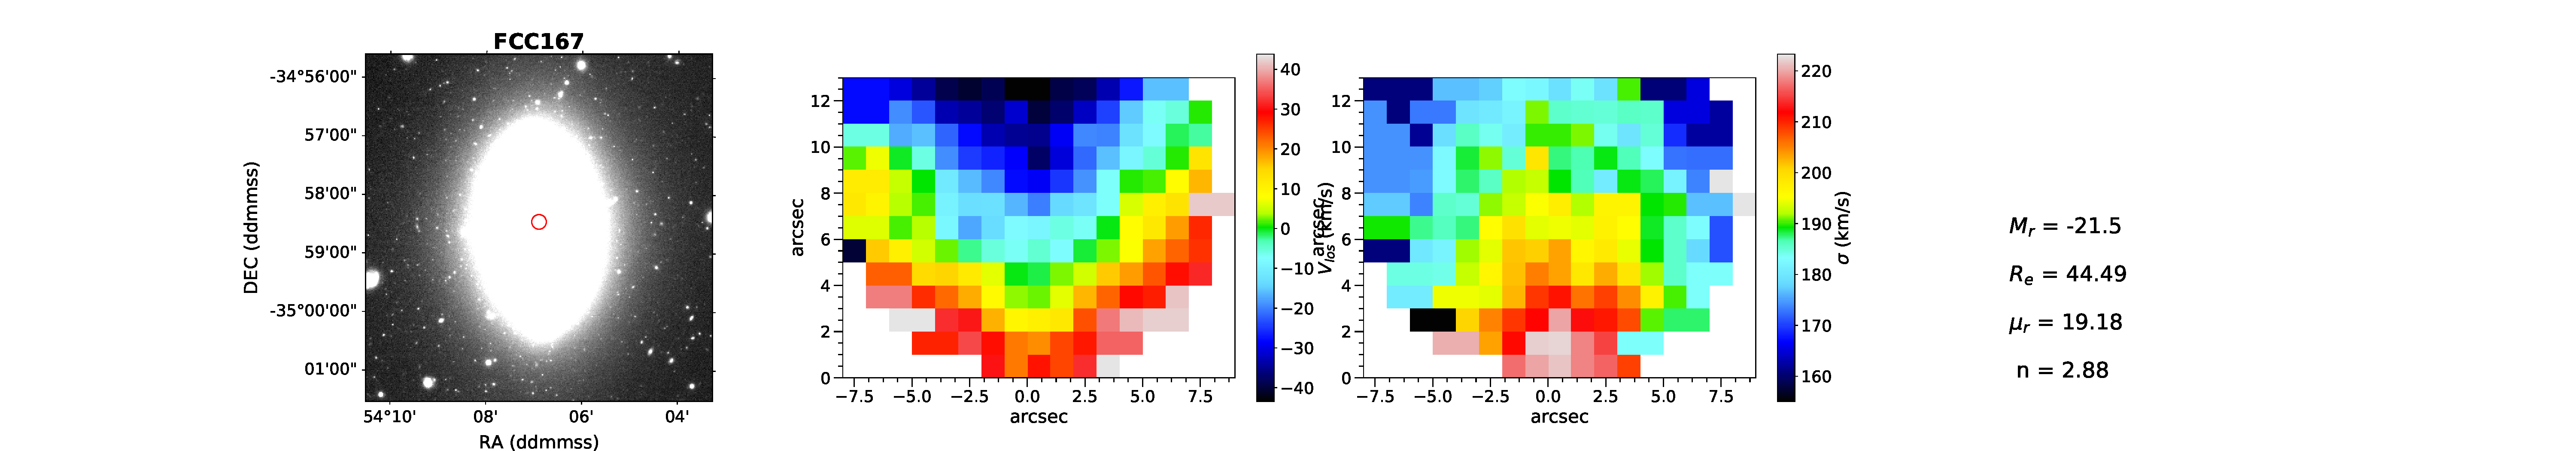
\includegraphics[width=21cm,height=6cm,keepaspectratio]{../2_pipeline/1_V&S_Maps/167Velocity_map.pdf}
   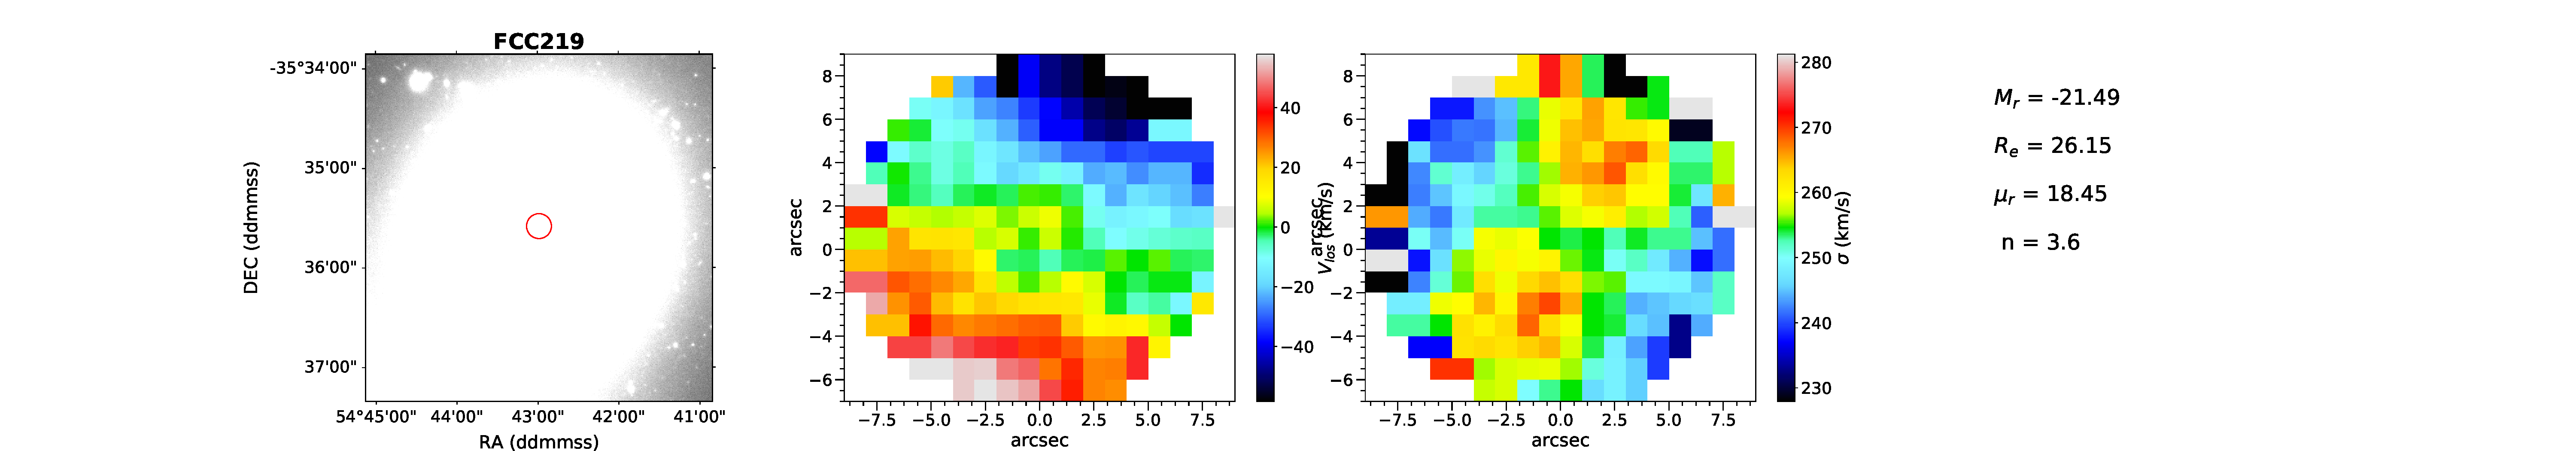
\includegraphics[width=21cm,height=6cm,keepaspectratio]{../2_pipeline/1_V&S_Maps/219Velocity_map.pdf}
   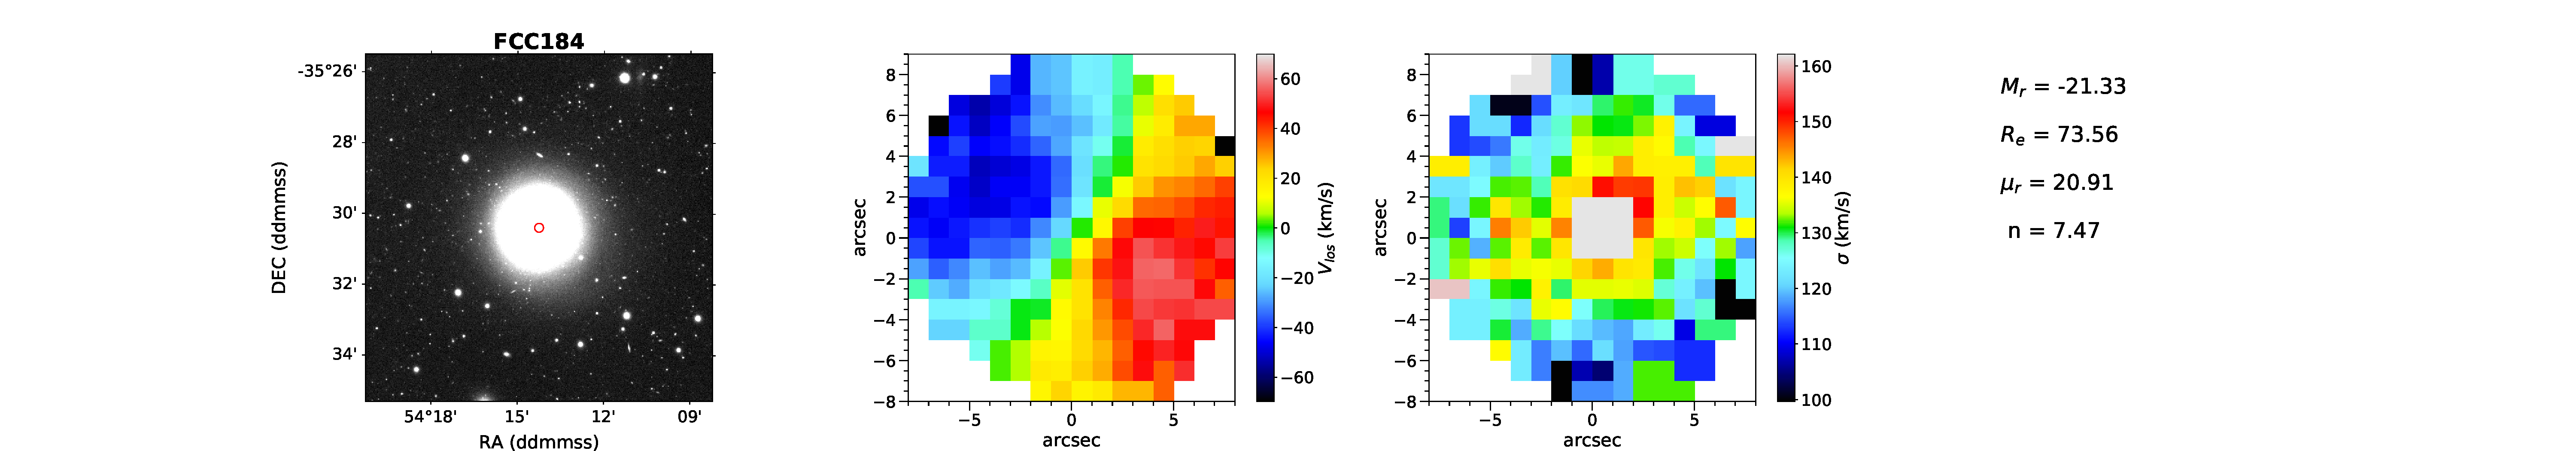
\includegraphics[width=21cm,height=6cm,keepaspectratio]{../2_pipeline/1_V&S_Maps/184Velocity_map.pdf}
   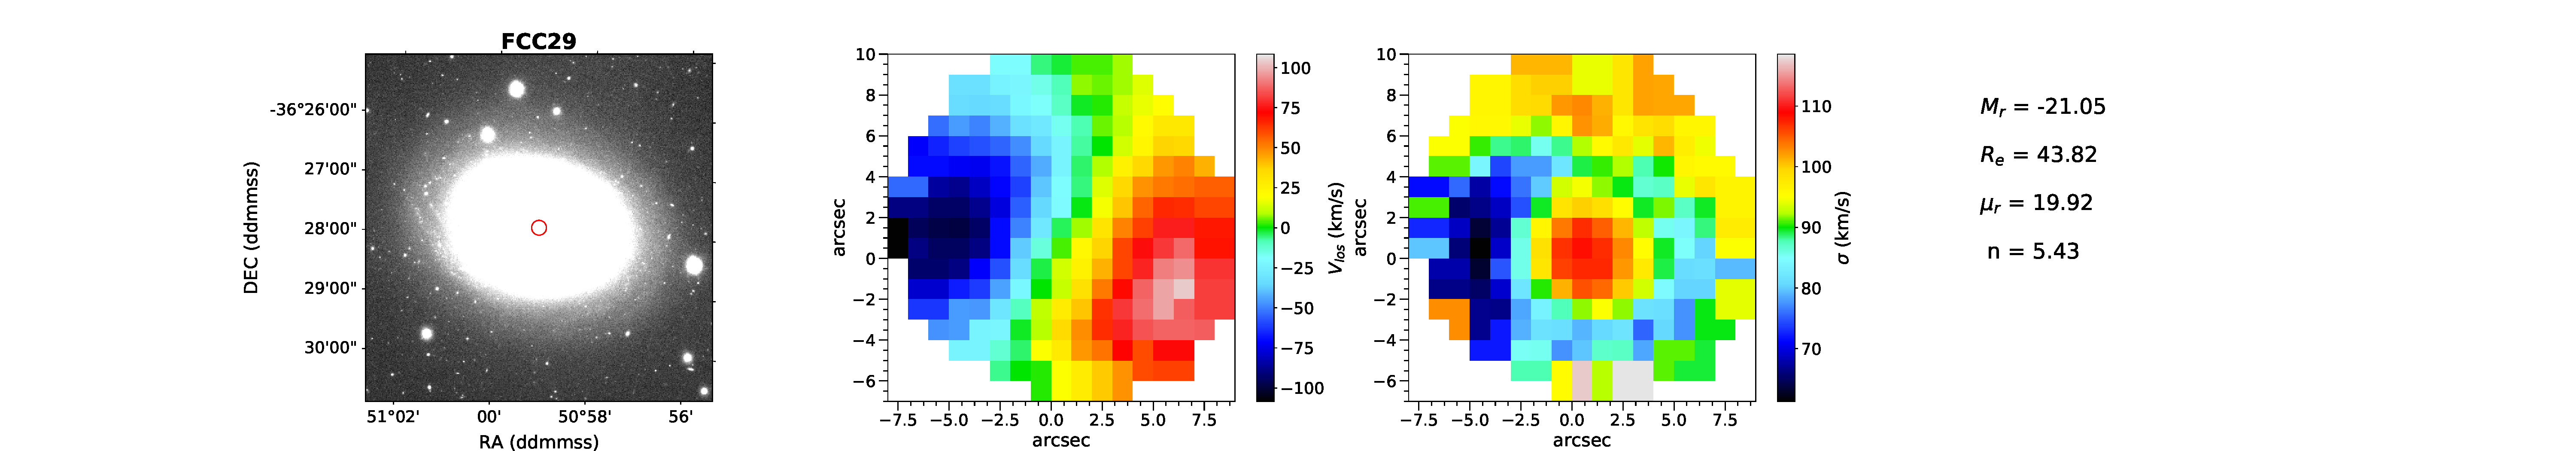
\includegraphics[width=21cm,height=6cm,keepaspectratio]
{../2_pipeline/1_V&S_Maps/29Velocity_map.pdf}
   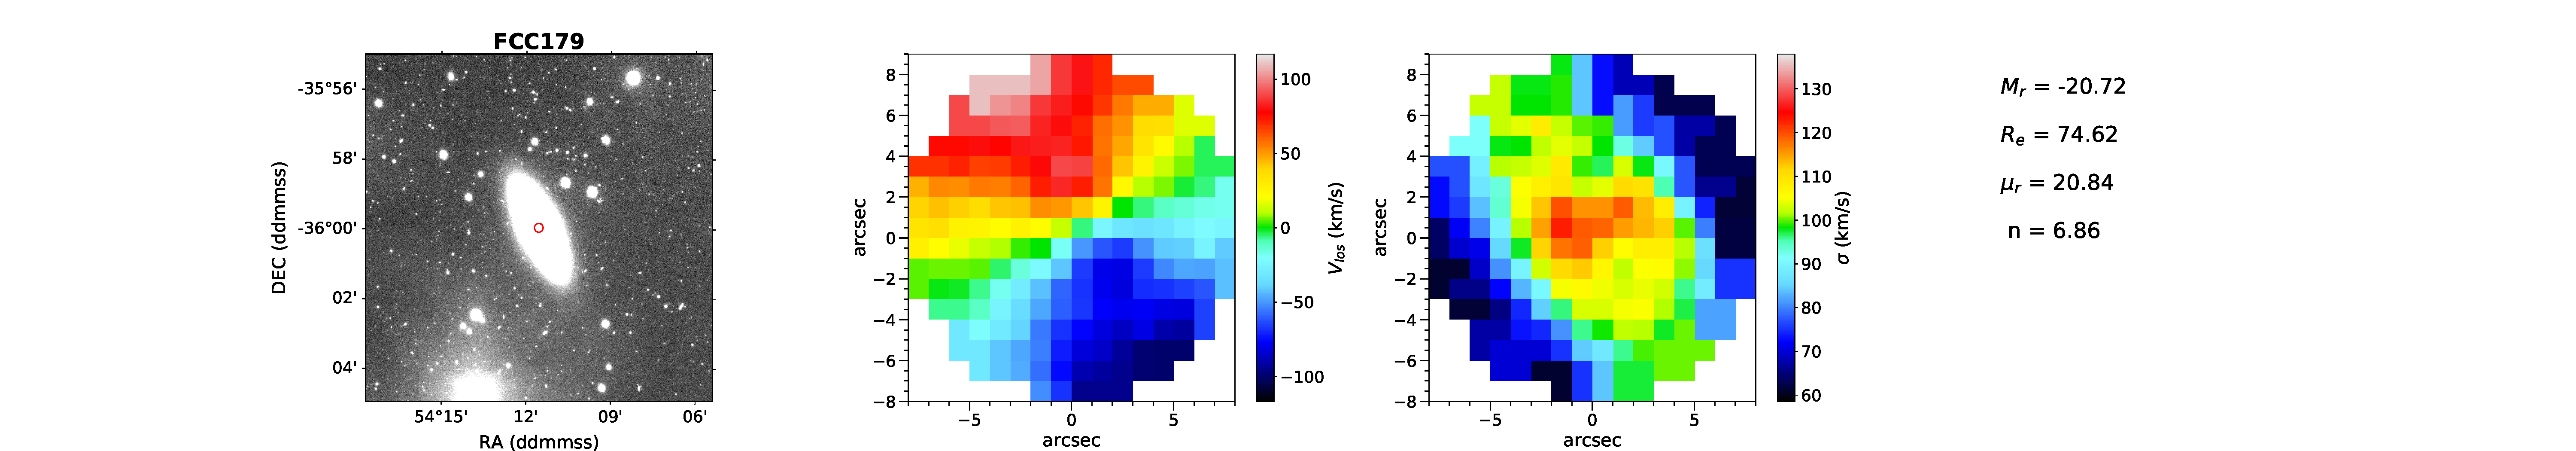
\includegraphics[width=21cm,height=6cm,keepaspectratio]
{../2_pipeline/1_V&S_Maps/179Velocity_map.pdf}
         \caption{Photometric images, Velocity maps, Dispersion maps}
         \label{FigVelDis}
\end{figure*}
\clearpage
%
\begin{figure*}[!htb]
   \ContinuedFloat
   \centering
   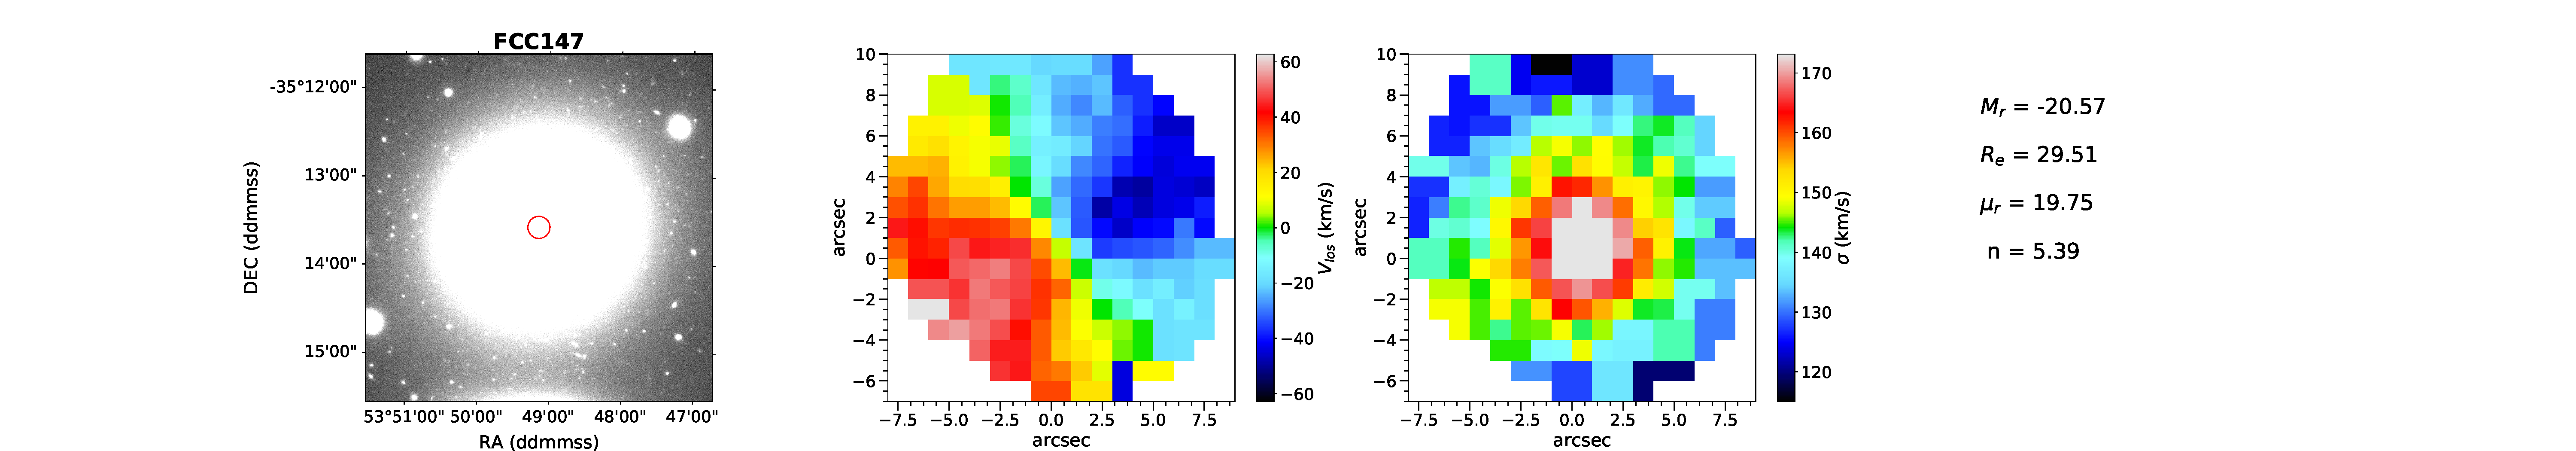
\includegraphics[width=21cm,height=6cm,keepaspectratio]
{../2_pipeline/1_V&S_Maps/147Velocity_map.pdf}
   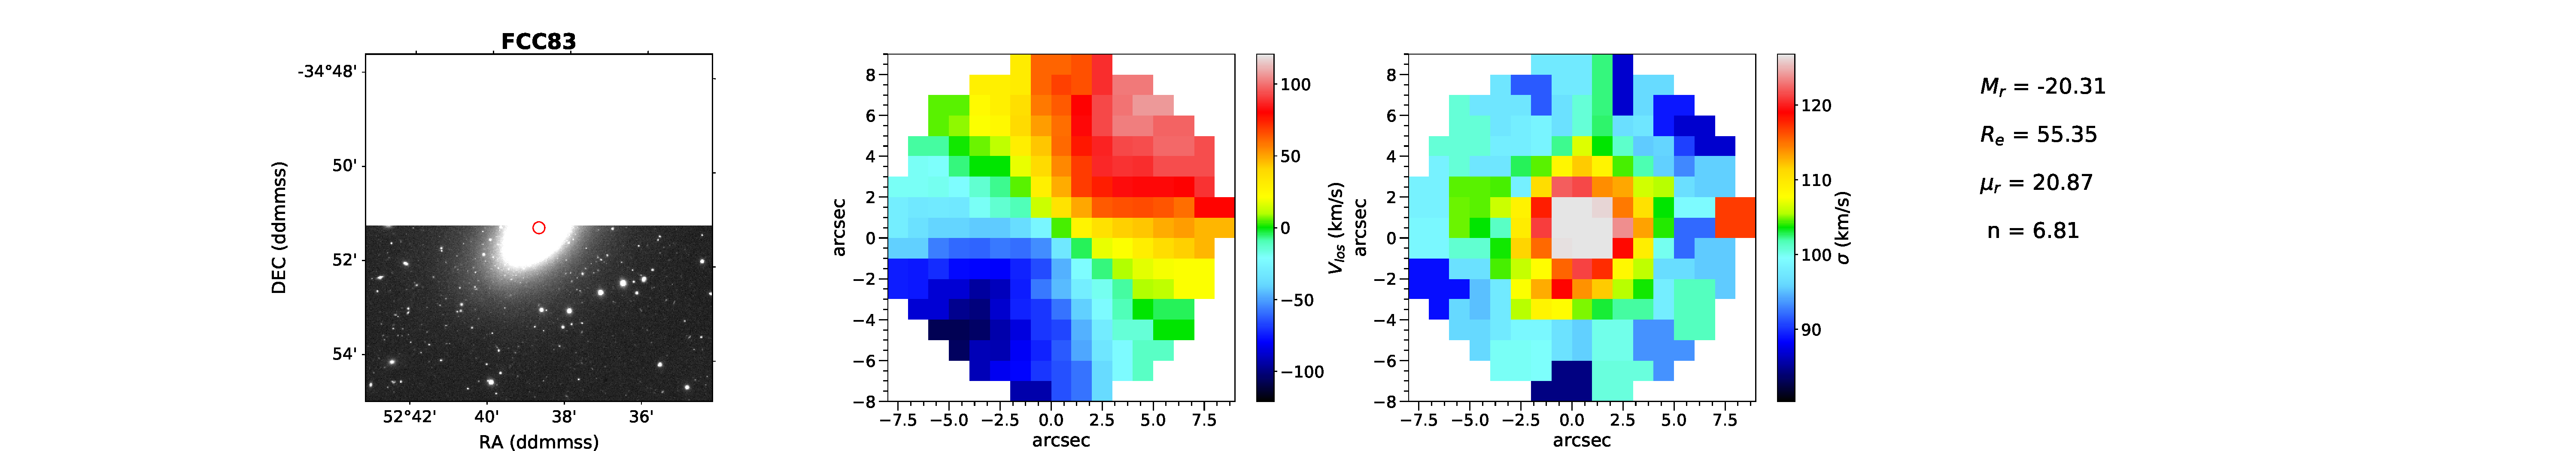
\includegraphics[width=21cm,height=6cm,keepaspectratio]{../2_pipeline/1_V&S_Maps/83Velocity_map.pdf}
   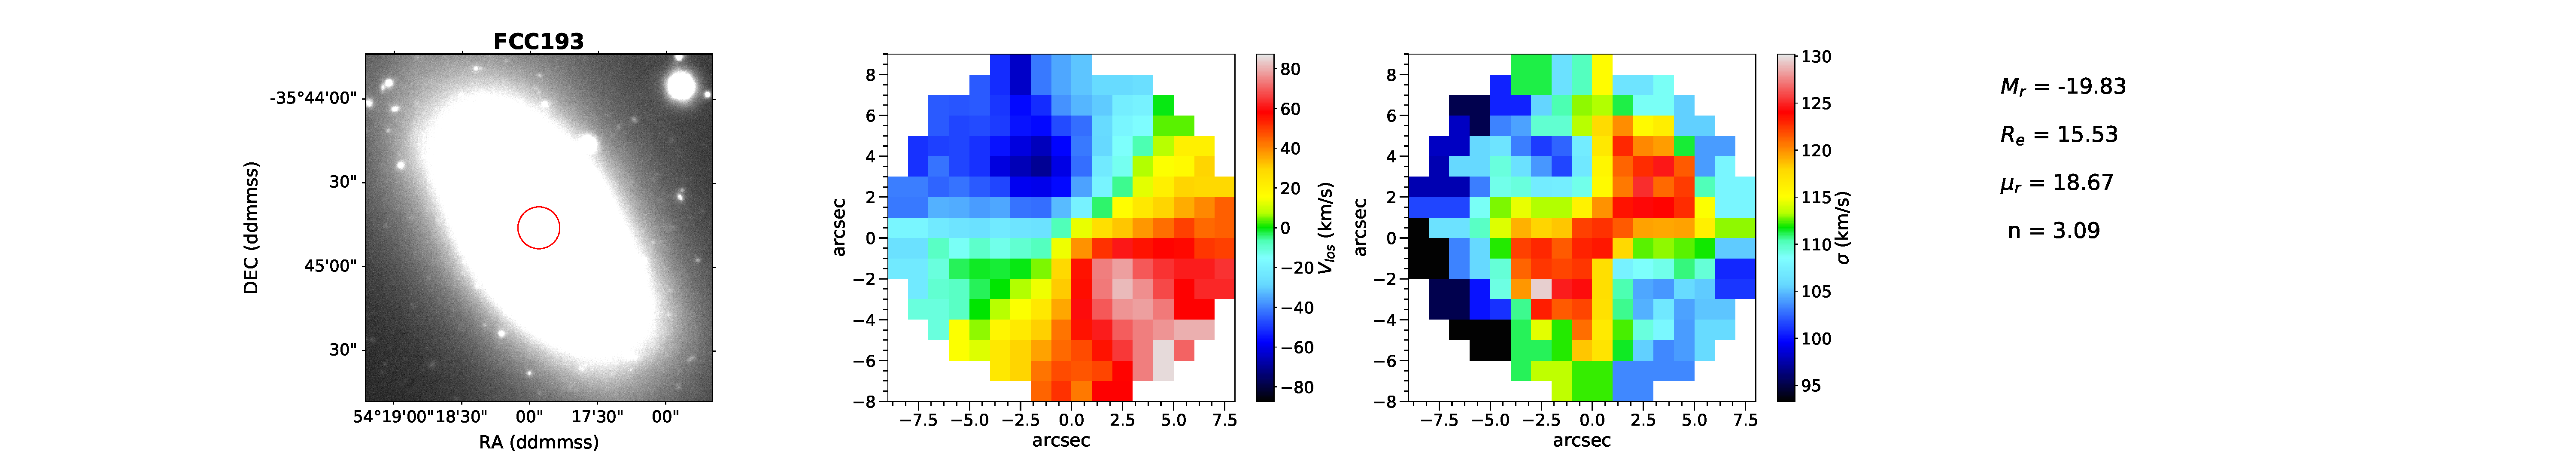
\includegraphics[width=21cm,height=6cm,keepaspectratio]{../2_pipeline/1_V&S_Maps/193Velocity_map.pdf}
   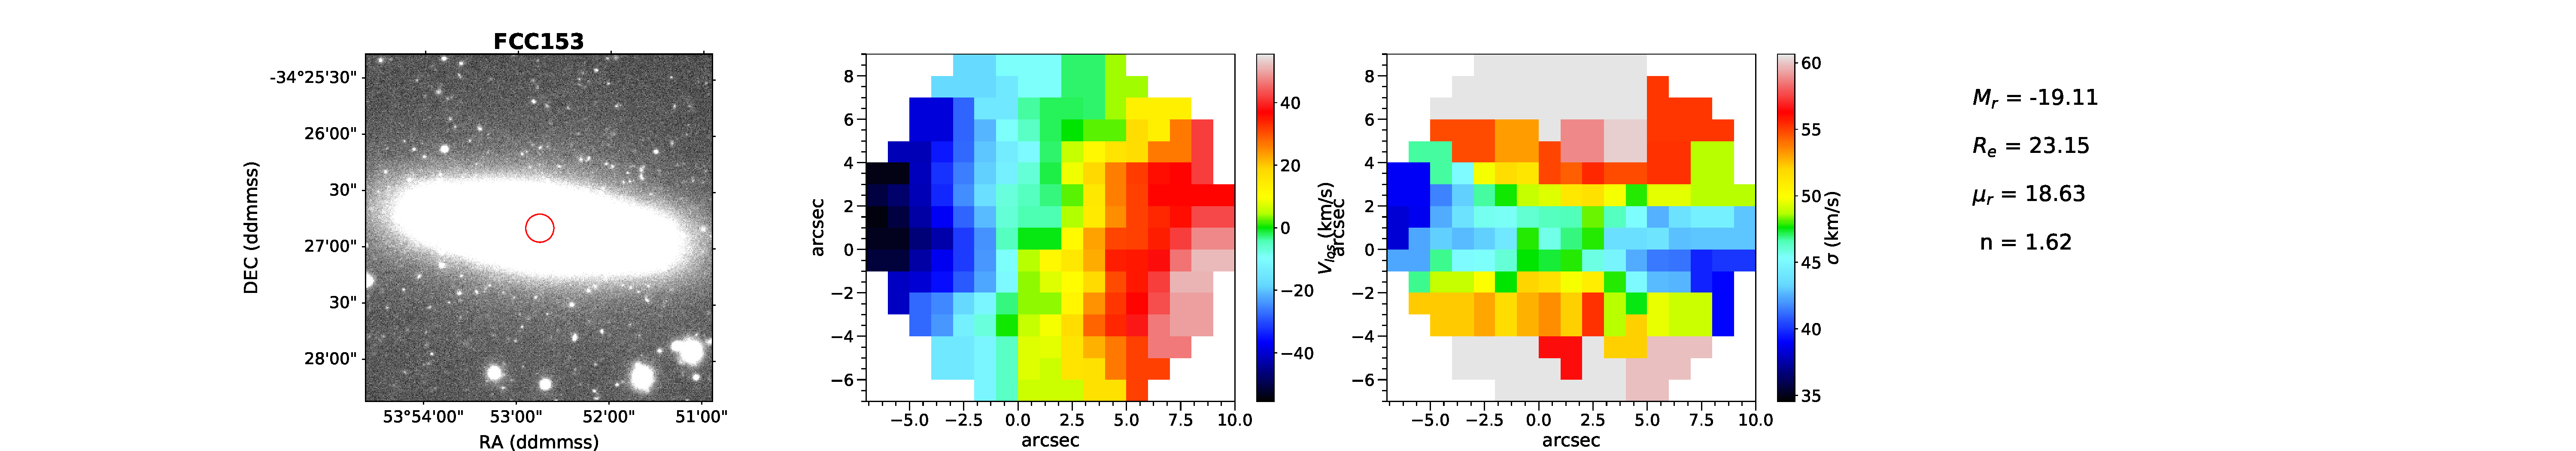
\includegraphics[width=21cm,height=6cm,keepaspectratio]{../2_pipeline/1_V&S_Maps/153Velocity_map.pdf}
   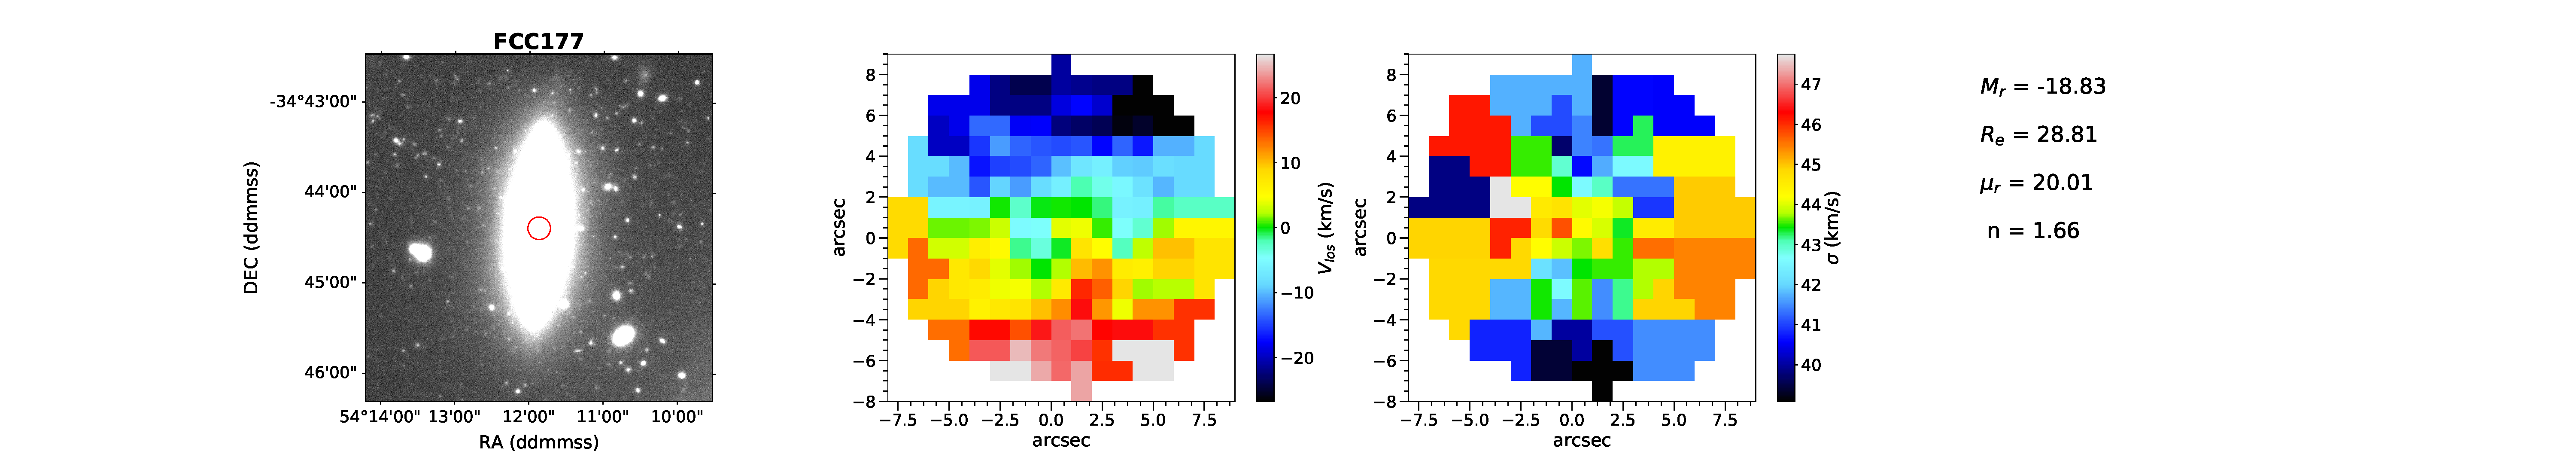
\includegraphics[width=21cm,height=6cm,keepaspectratio]{../2_pipeline/1_V&S_Maps/177Velocity_map.pdf}
   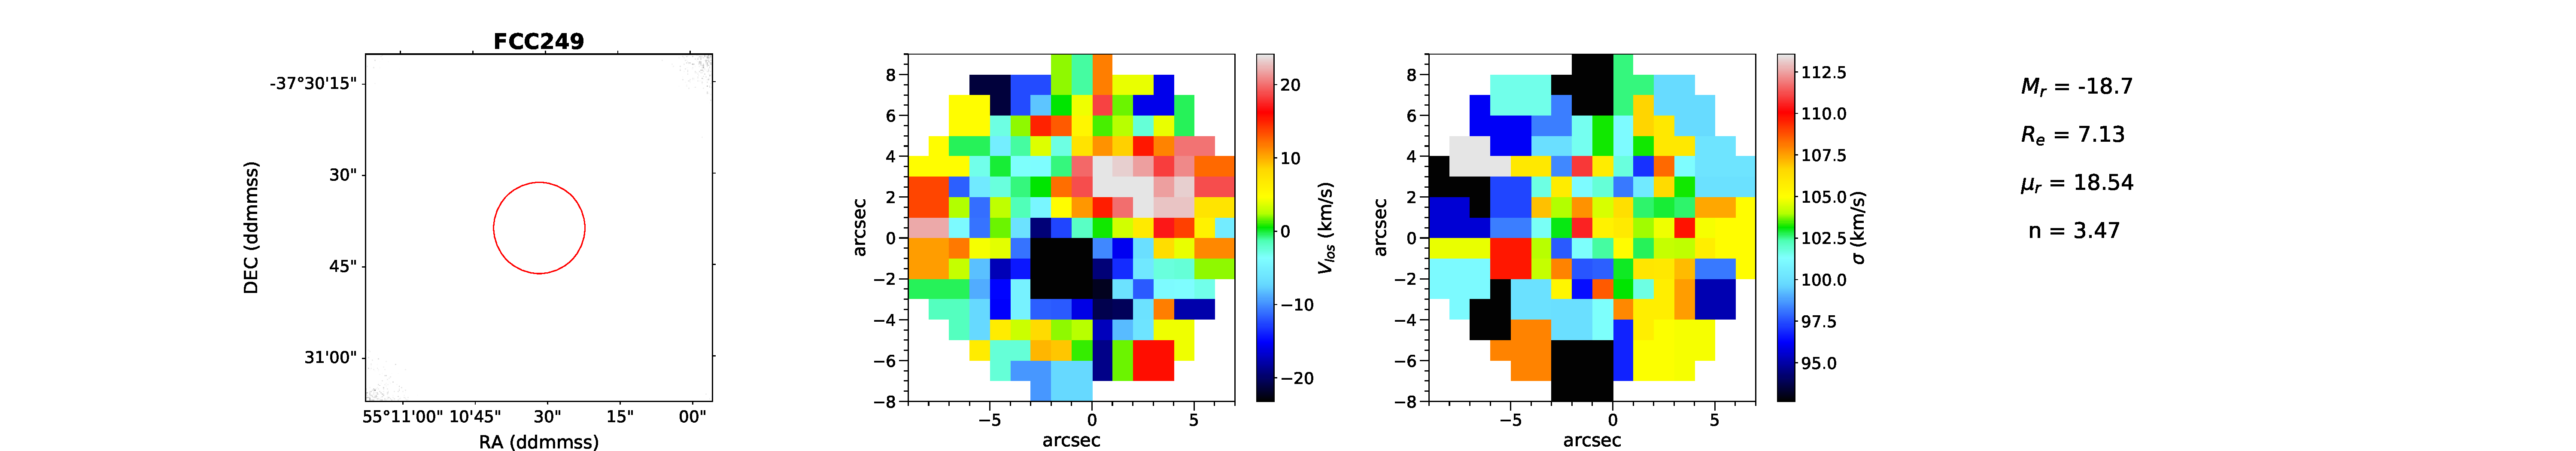
\includegraphics[width=21cm,height=6cm,keepaspectratio]{../2_pipeline/1_V&S_Maps/249Velocity_map.pdf}
         \caption{Photometric images, Velocity maps, Dispersion maps}
         \label{FigVelDis}
\end{figure*}
\clearpage
%
\begin{figure*}[!htb]
   \ContinuedFloat
   \centering
   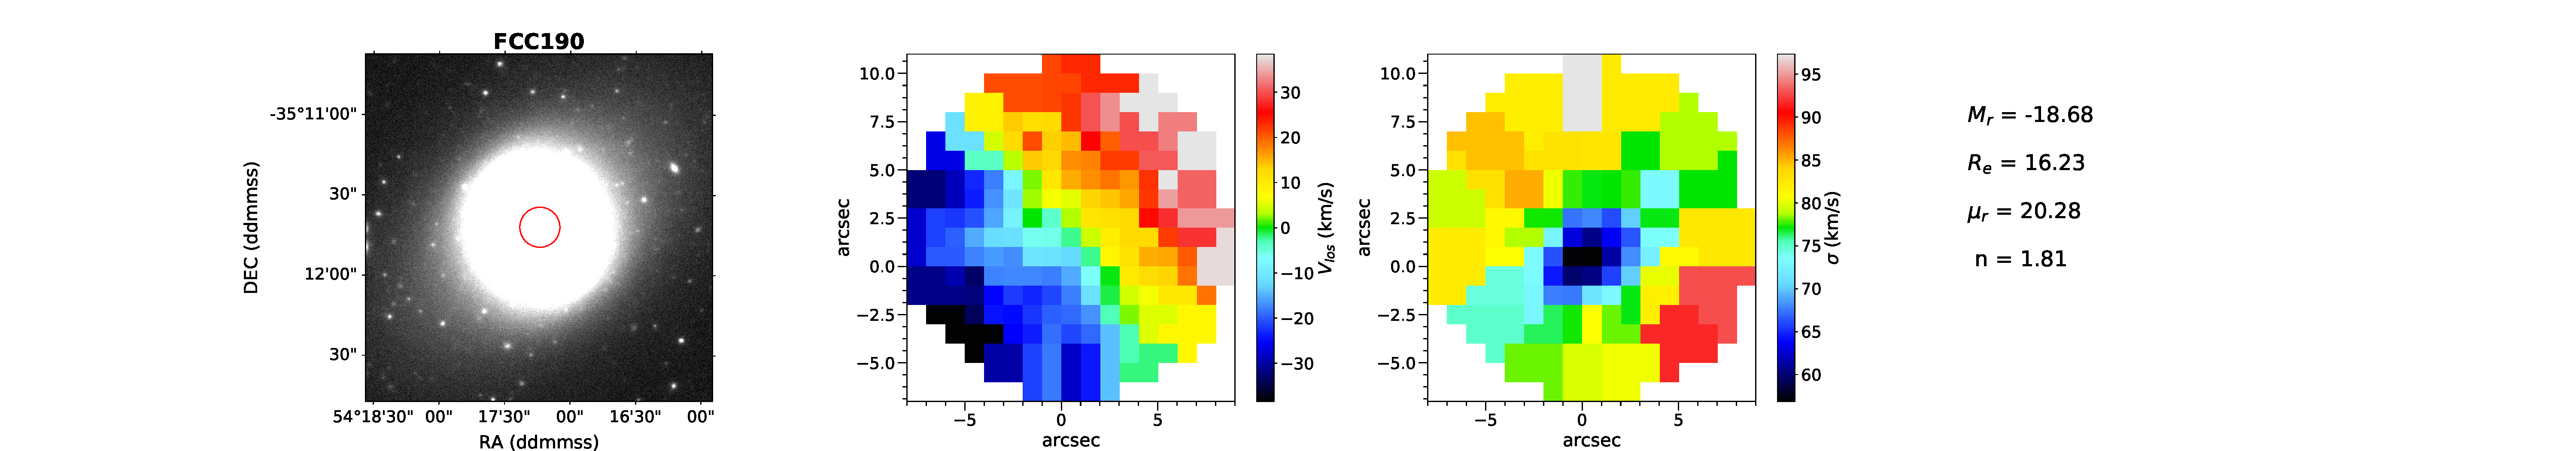
\includegraphics[width=21cm,height=6cm,keepaspectratio]{../2_pipeline/1_V&S_Maps/190Velocity_map.pdf}
   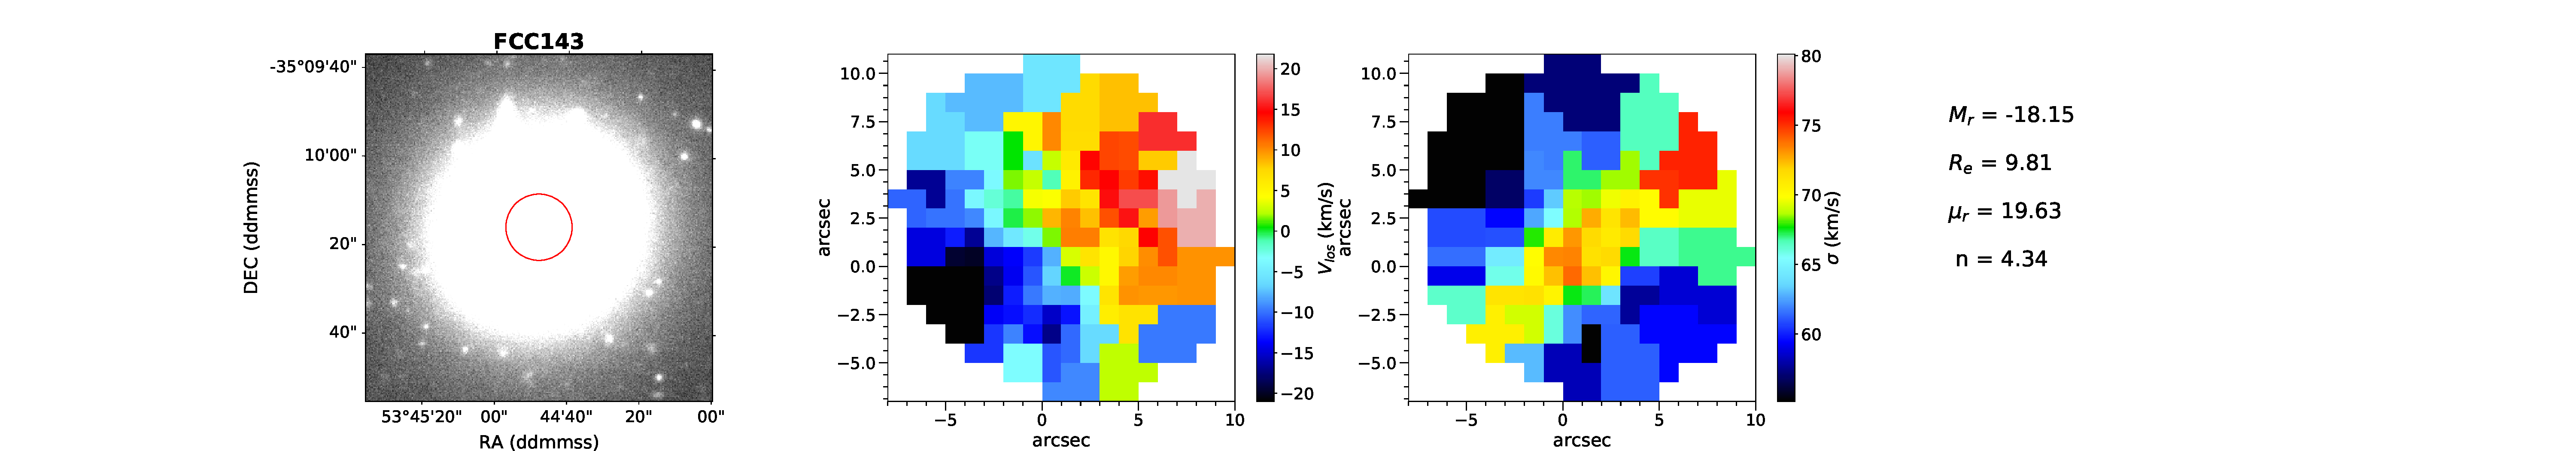
\includegraphics[width=21cm,height=6cm,keepaspectratio]{../2_pipeline/1_V&S_Maps/143Velocity_map.pdf}
   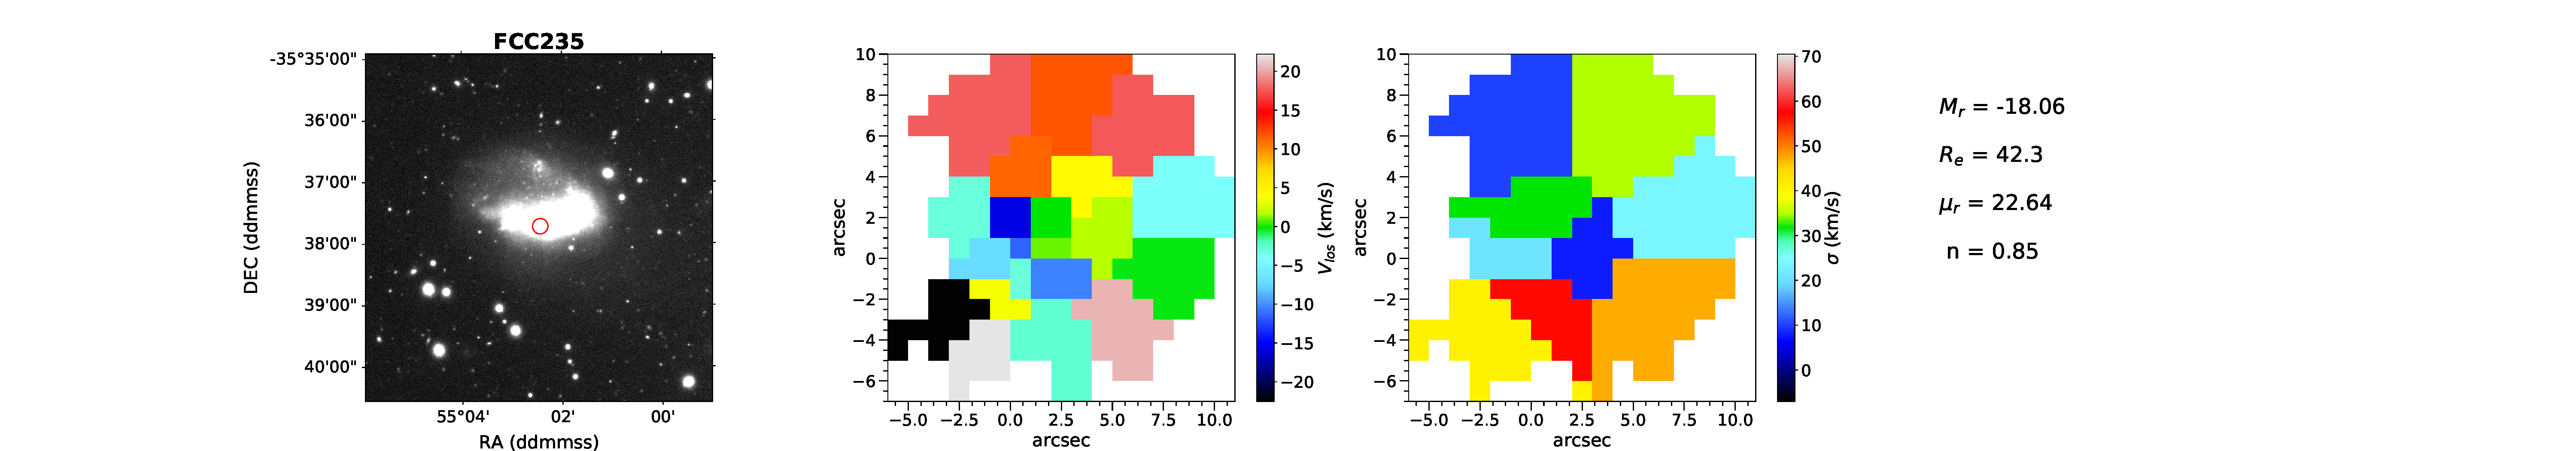
\includegraphics[width=21cm,height=6cm,keepaspectratio]{../2_pipeline/1_V&S_Maps/235Velocity_map.pdf}
   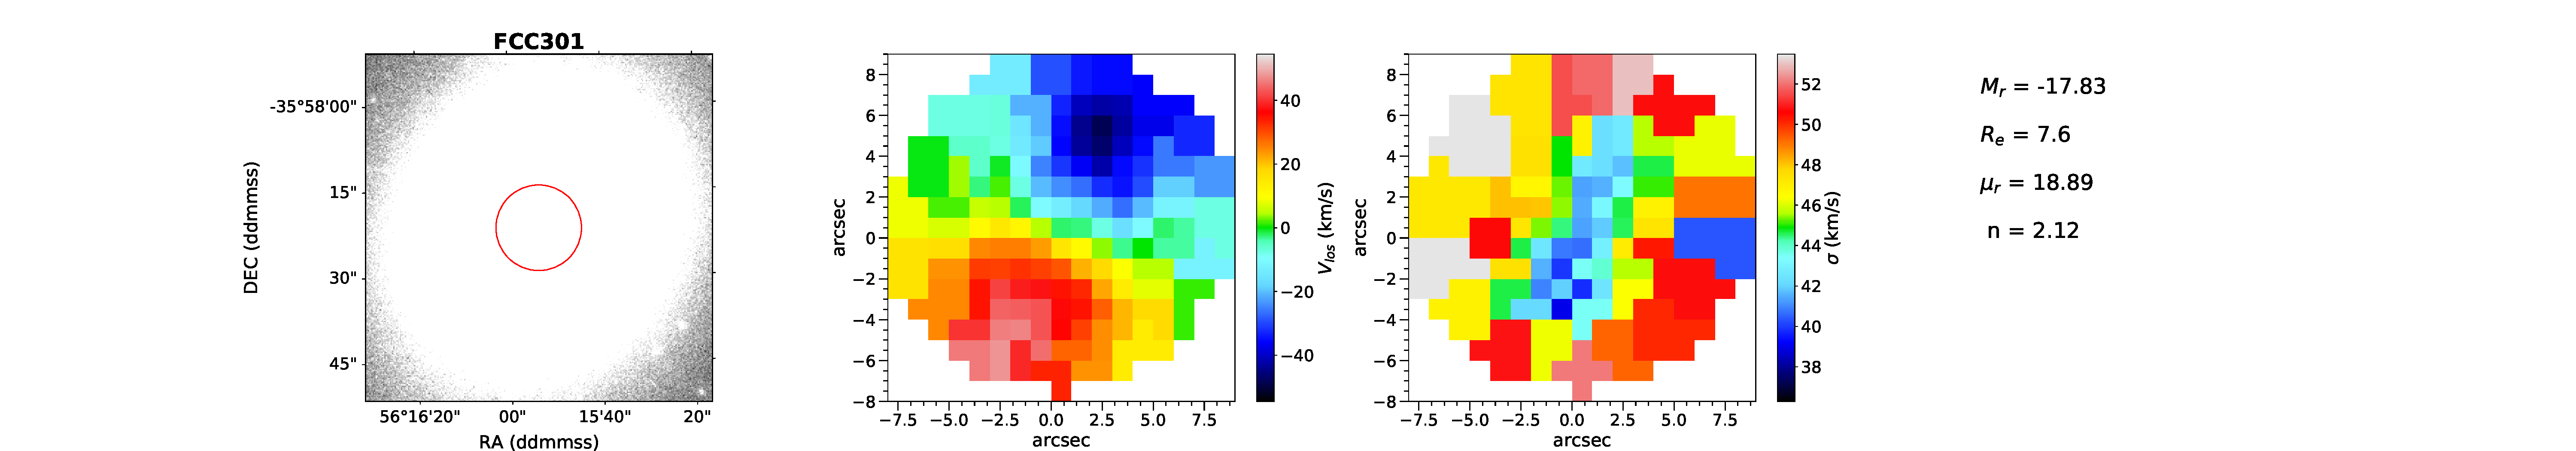
\includegraphics[width=21cm,height=6cm,keepaspectratio]{../2_pipeline/1_V&S_Maps/301Velocity_map.pdf}
   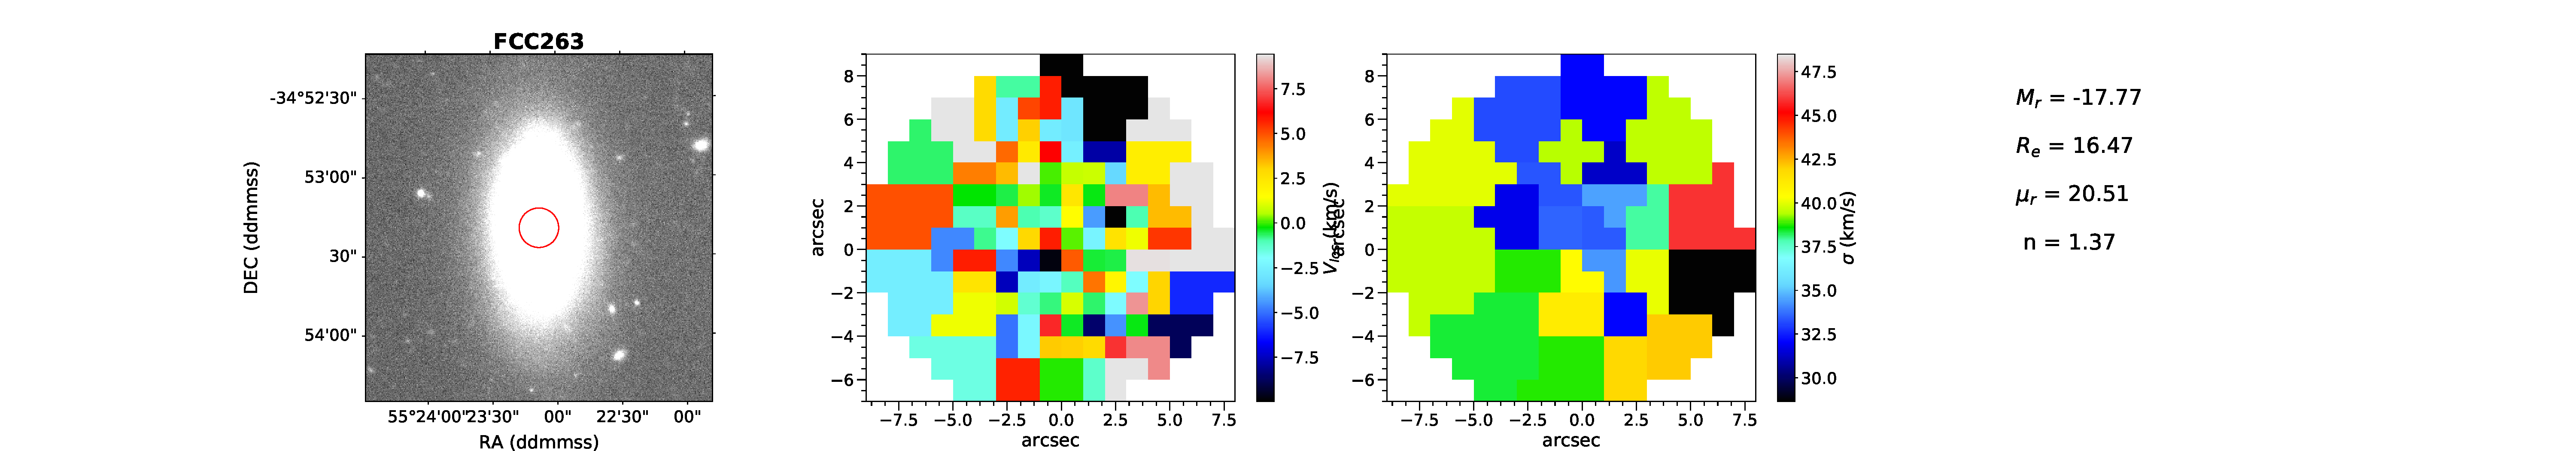
\includegraphics[width=21cm,height=6cm,keepaspectratio]{../2_pipeline/1_V&S_Maps/263Velocity_map.pdf}
   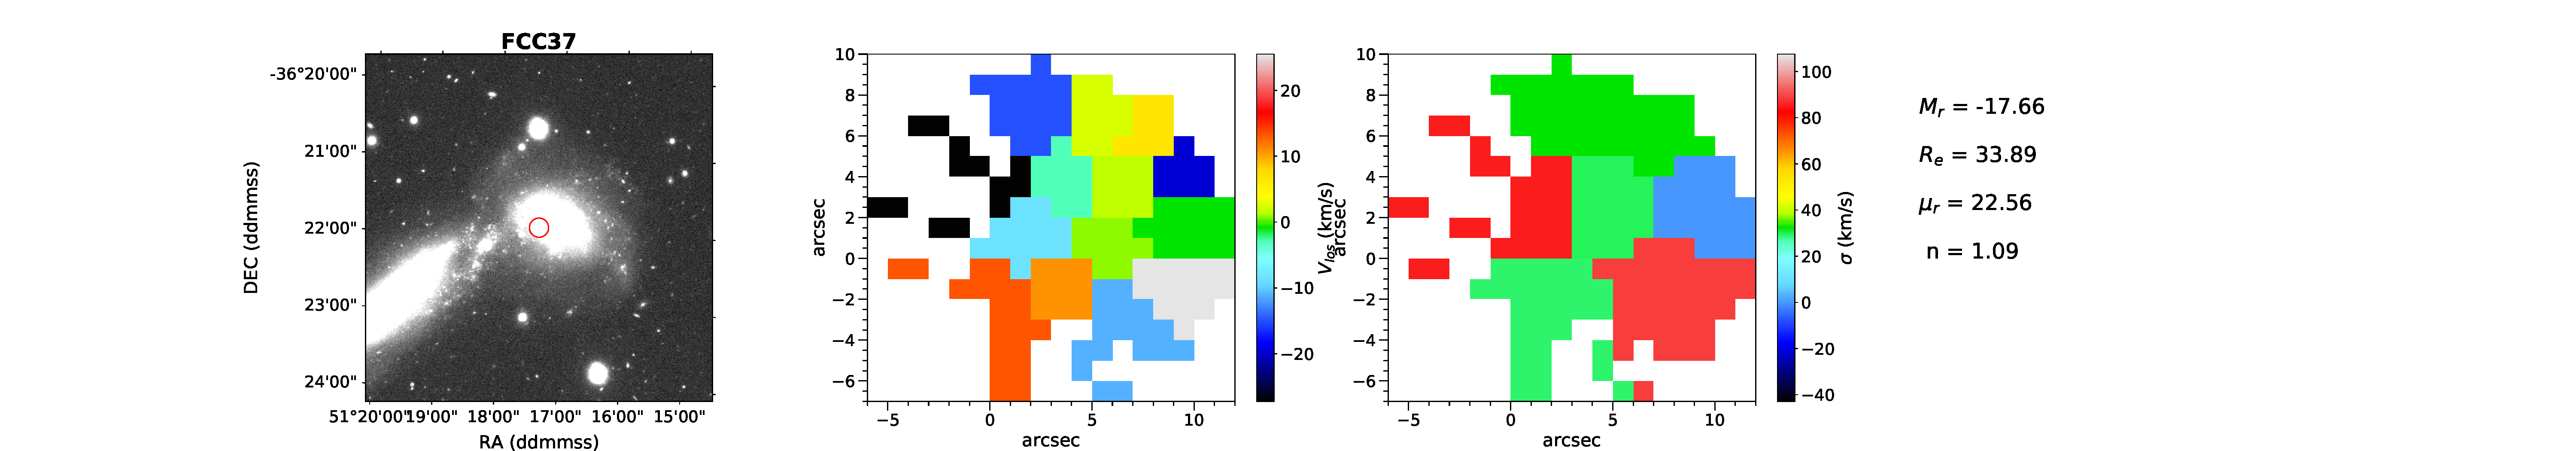
\includegraphics[width=21cm,height=6cm,keepaspectratio]{../2_pipeline/1_V&S_Maps/37Velocity_map.pdf}
         \caption{Photometric images, Velocity maps, Dispersion maps}
         \label{FigVelDis}
\end{figure*}
\clearpage
%
\begin{figure*}[!htb]
   \ContinuedFloat
   \centering
   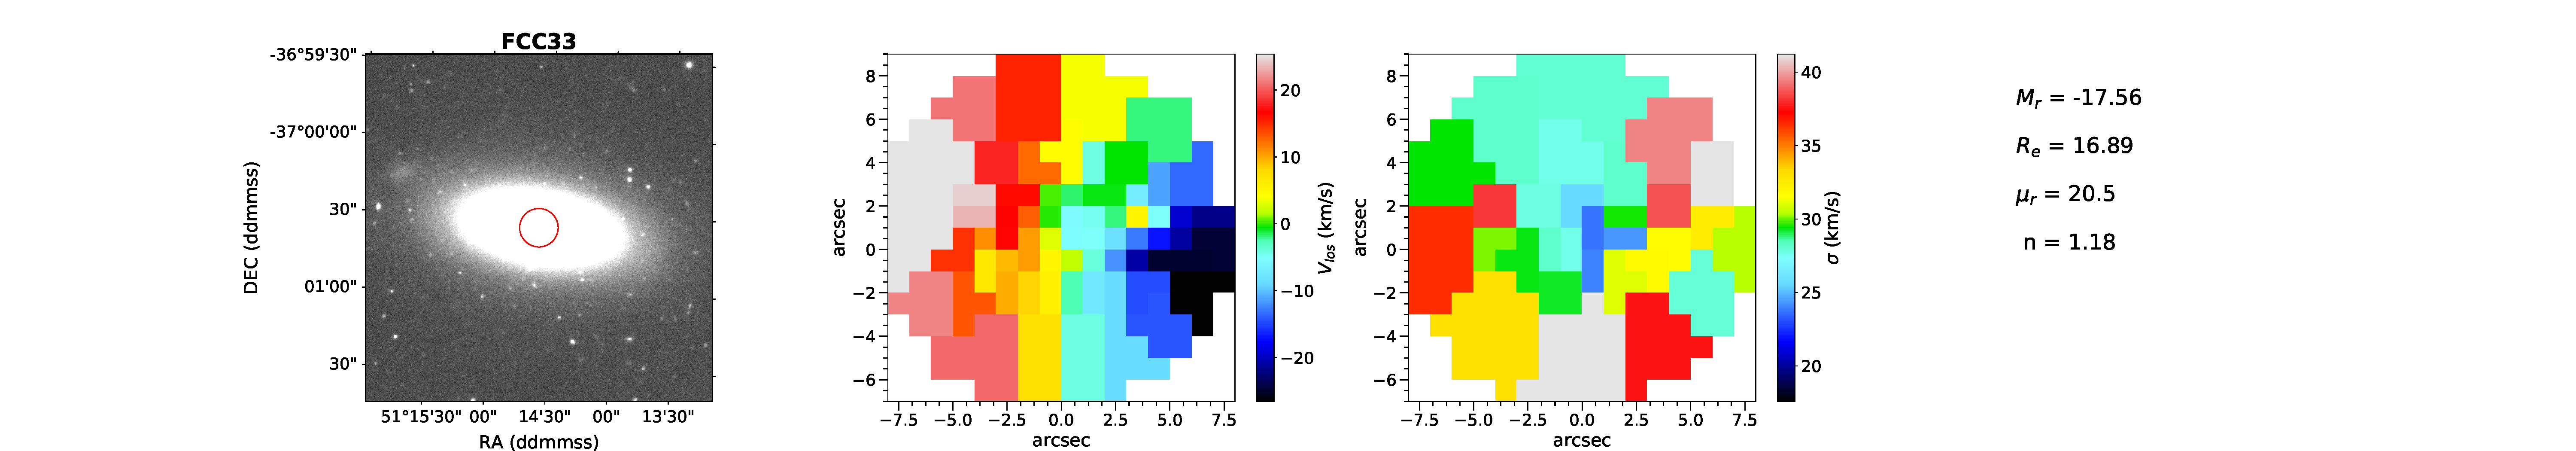
\includegraphics[width=21cm,height=6cm,keepaspectratio]{../2_pipeline/1_V&S_Maps/33Velocity_map.pdf}
   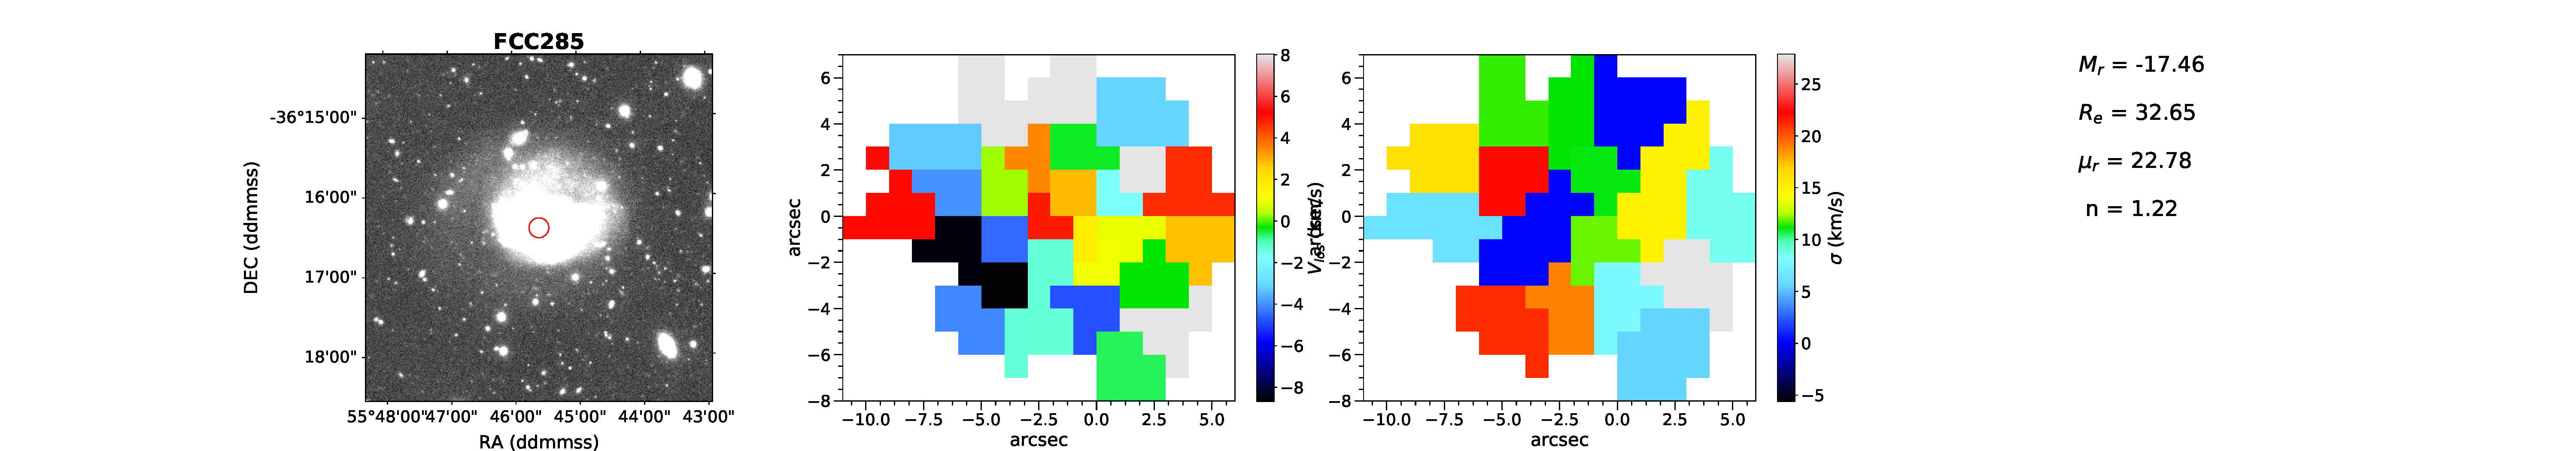
\includegraphics[width=21cm,height=6cm,keepaspectratio]{../2_pipeline/1_V&S_Maps/285Velocity_map.pdf}
   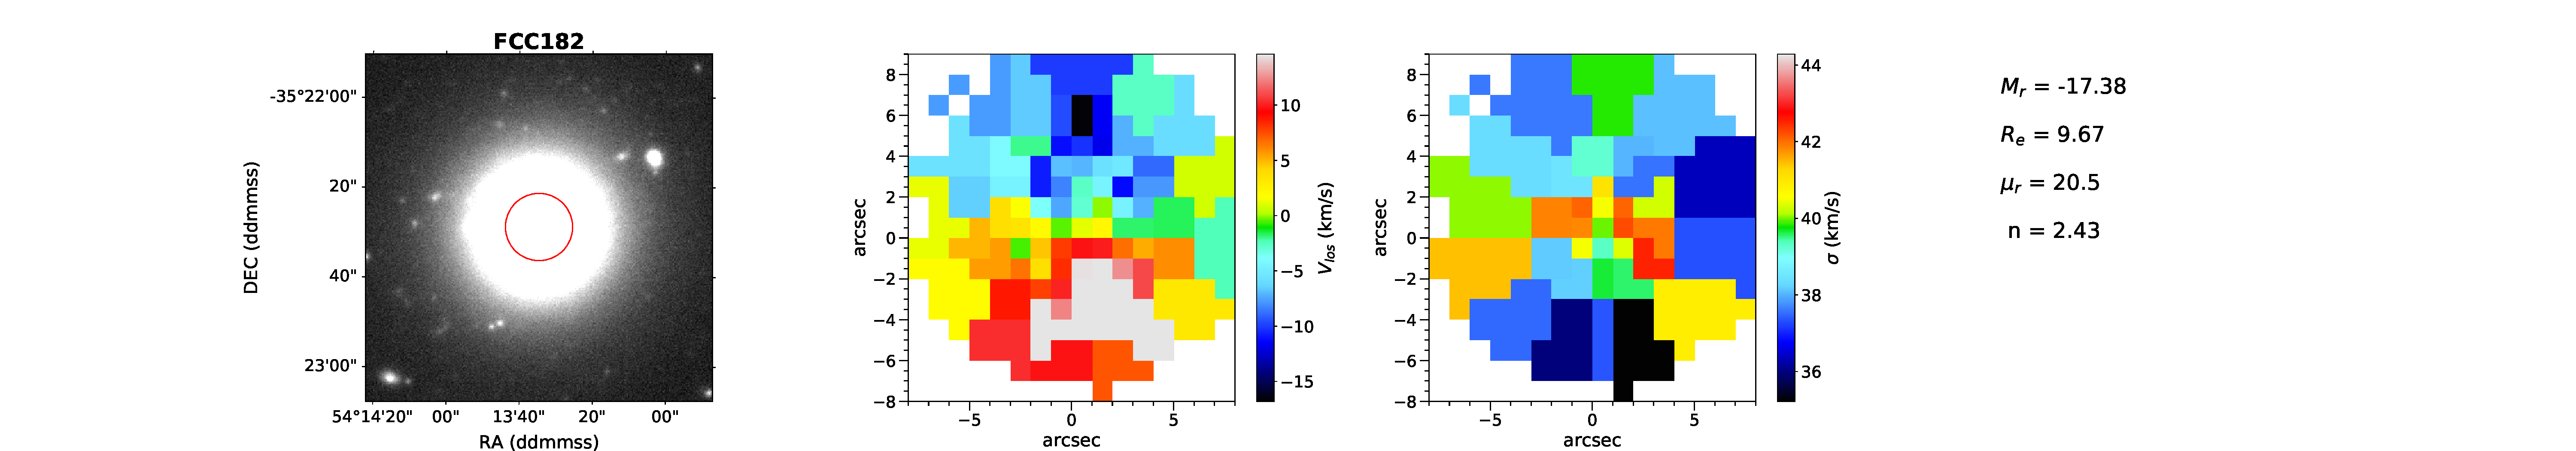
\includegraphics[width=21cm,height=6cm,keepaspectratio]{../2_pipeline/1_V&S_Maps/182Velocity_map.pdf}
   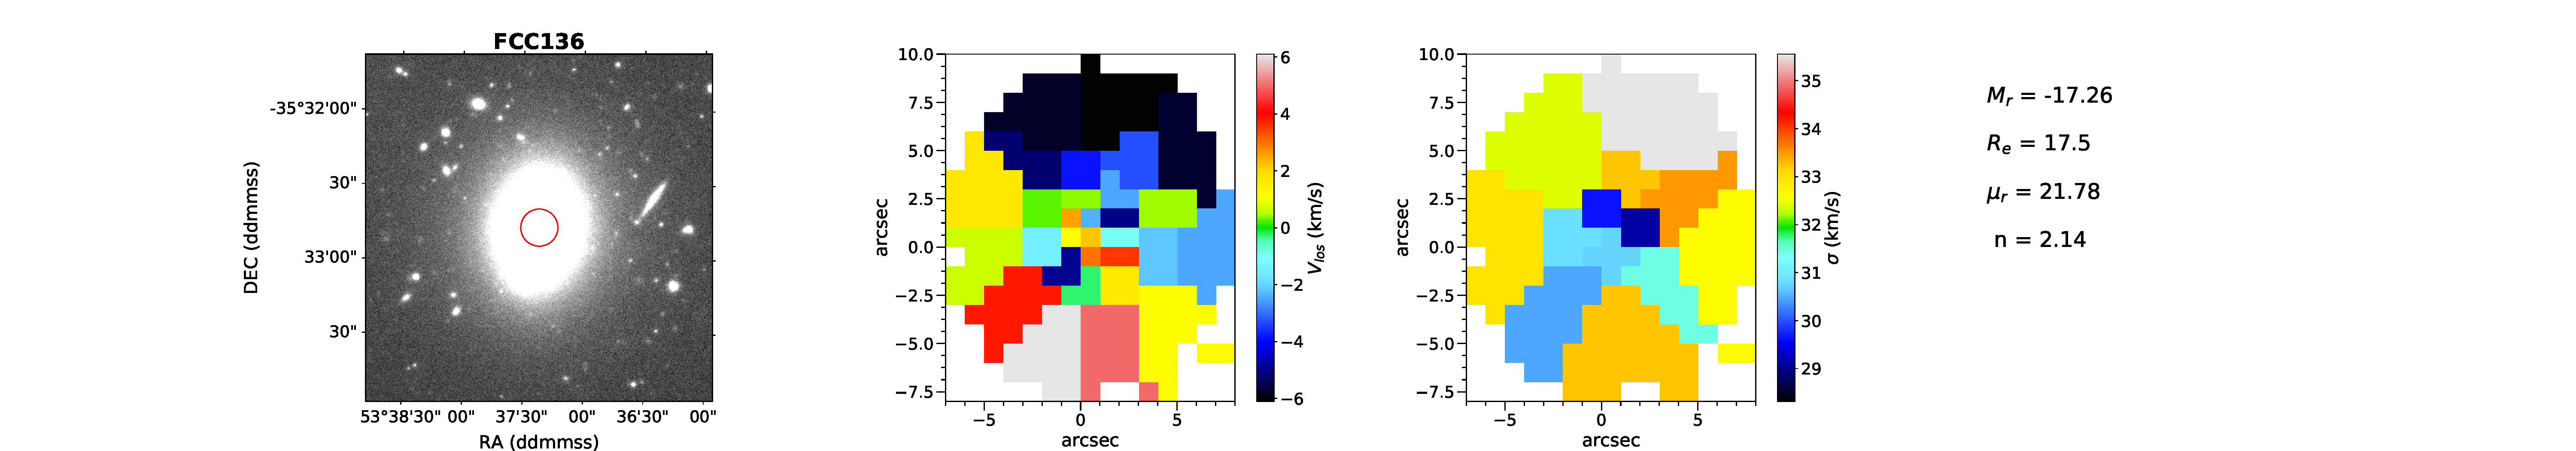
\includegraphics[width=21cm,height=6cm,keepaspectratio]{../2_pipeline/1_V&S_Maps/136Velocity_map.pdf}
   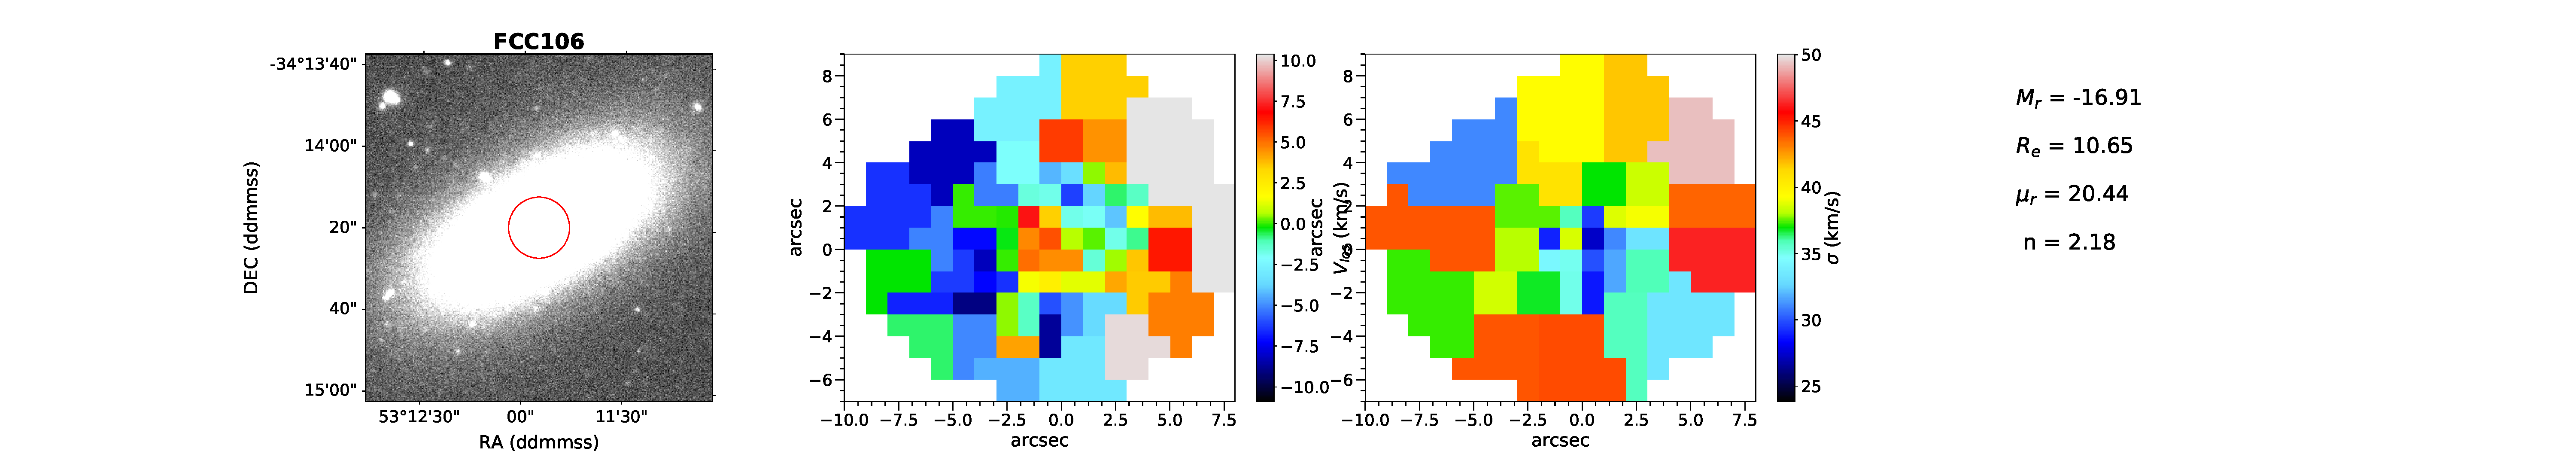
\includegraphics[width=21cm,height=6cm,keepaspectratio]{../2_pipeline/1_V&S_Maps/106Velocity_map.pdf}
   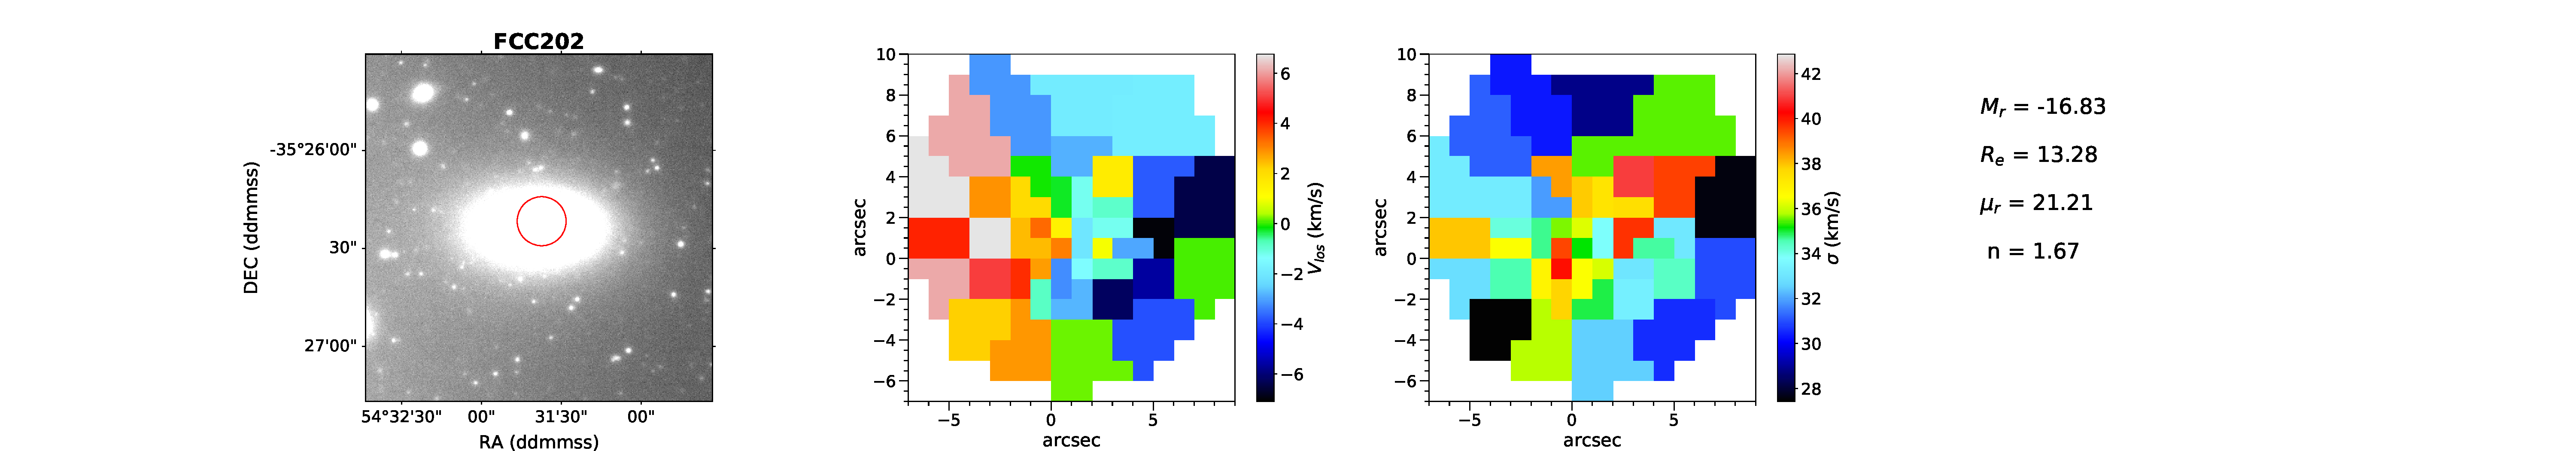
\includegraphics[width=21cm,height=6cm,keepaspectratio]{../2_pipeline/1_V&S_Maps/202Velocity_map.pdf}
         \caption{Photometric images, Velocity maps, Dispersion maps}
         \label{FigVelDis}
\end{figure*}
\clearpage
%
\begin{figure*}[!htb]
   \ContinuedFloat
   \centering
   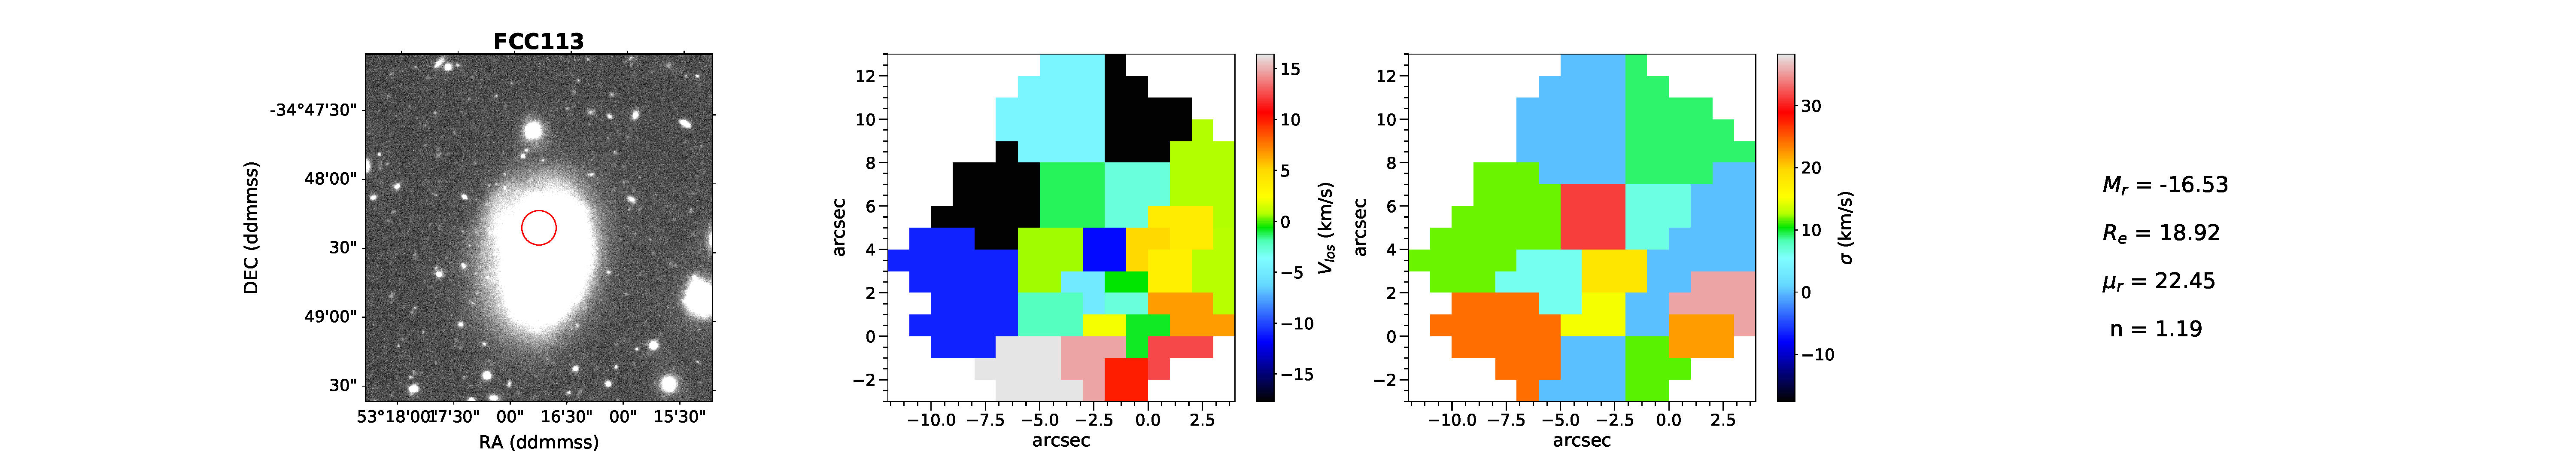
\includegraphics[width=21cm,height=6cm,keepaspectratio]{../2_pipeline/1_V&S_Maps/113Velocity_map.pdf}
   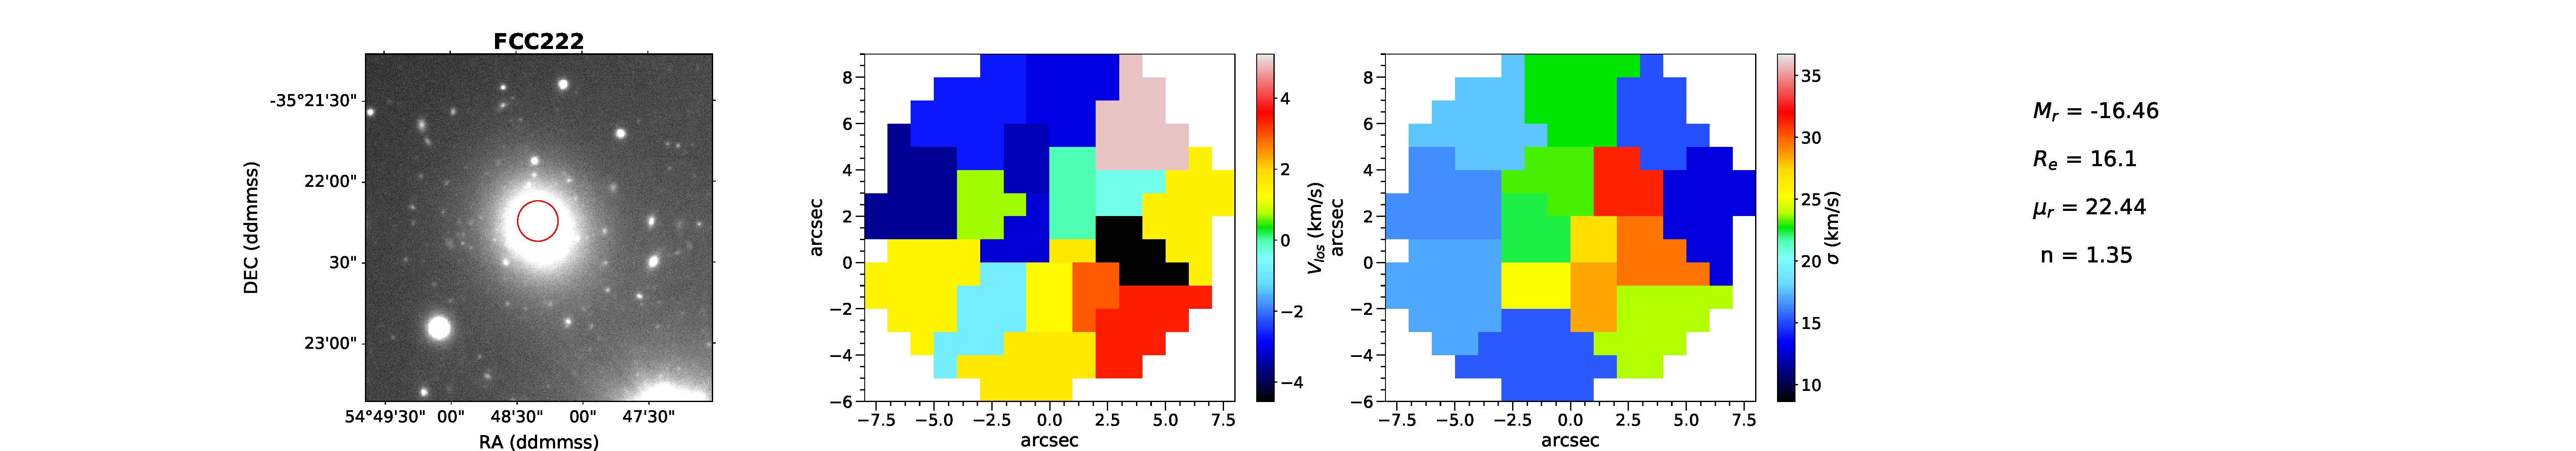
\includegraphics[width=21cm,height=6cm,keepaspectratio]{../2_pipeline/1_V&S_Maps/222Velocity_map.pdf}
   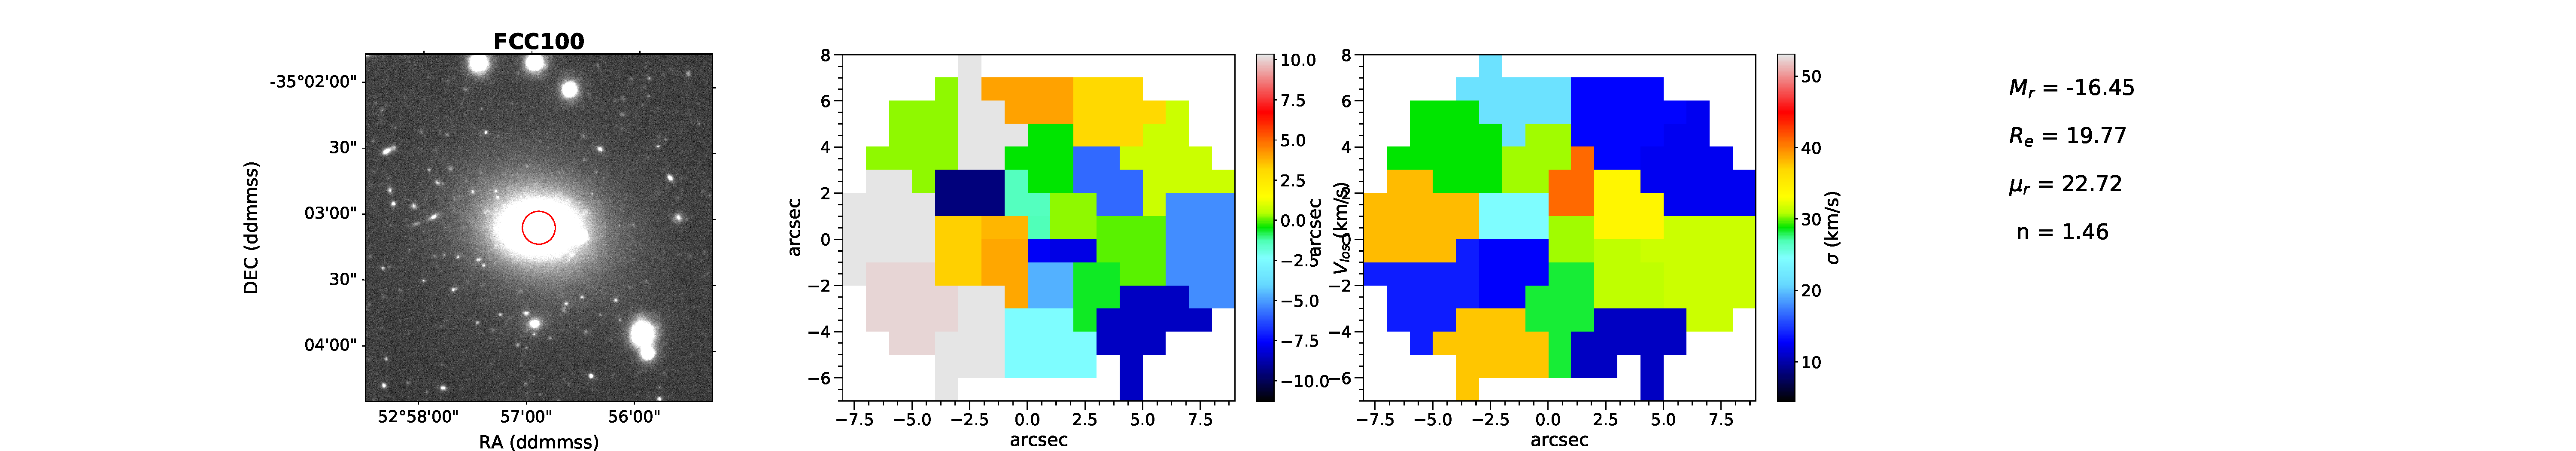
\includegraphics[width=21cm,height=6cm,keepaspectratio]{../2_pipeline/1_V&S_Maps/100Velocity_map.pdf}
   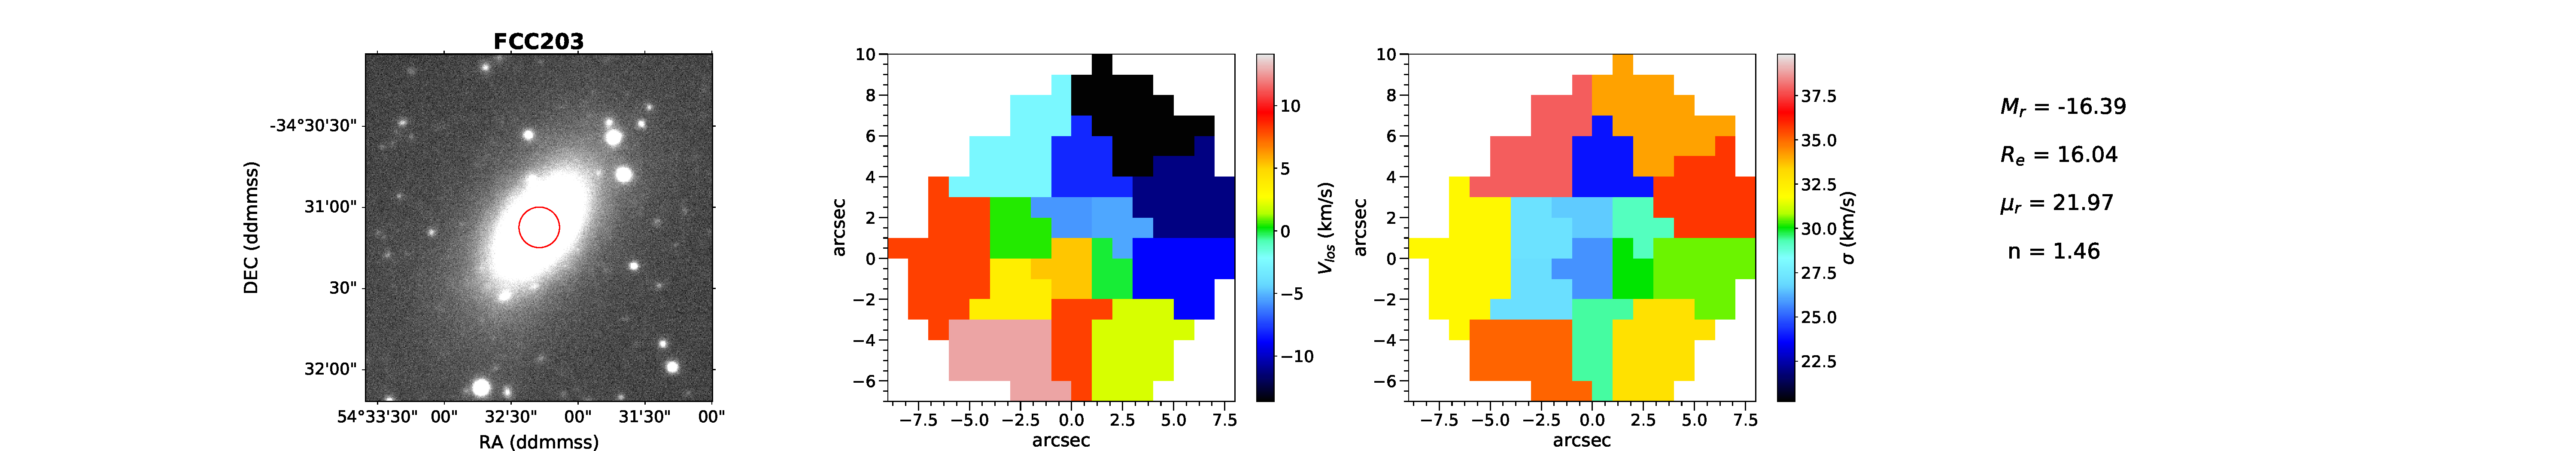
\includegraphics[width=21cm,height=6cm,keepaspectratio]{../2_pipeline/1_V&S_Maps/203Velocity_map.pdf}
   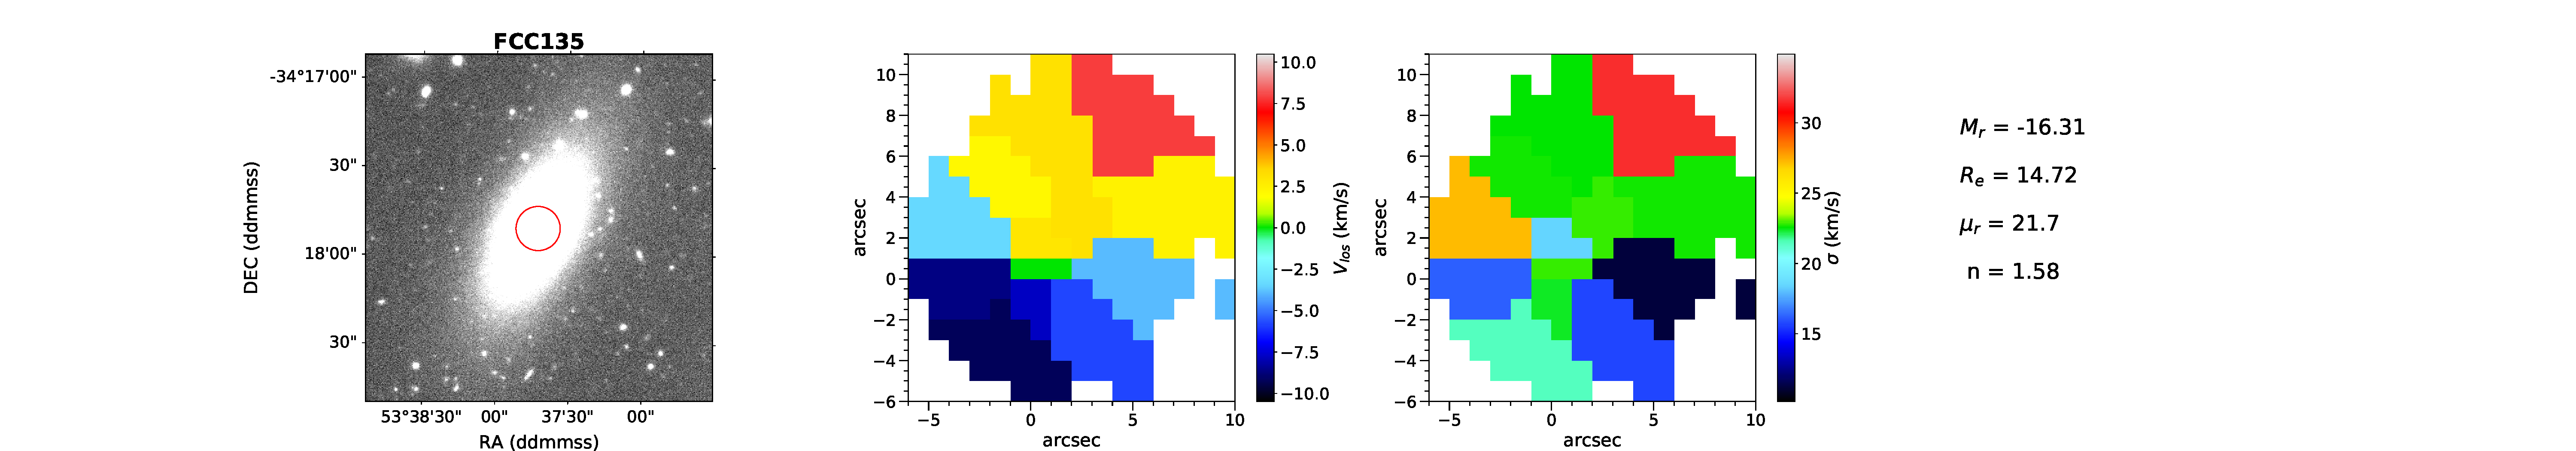
\includegraphics[width=21cm,height=6cm,keepaspectratio]{../2_pipeline/1_V&S_Maps/135Velocity_map.pdf}
   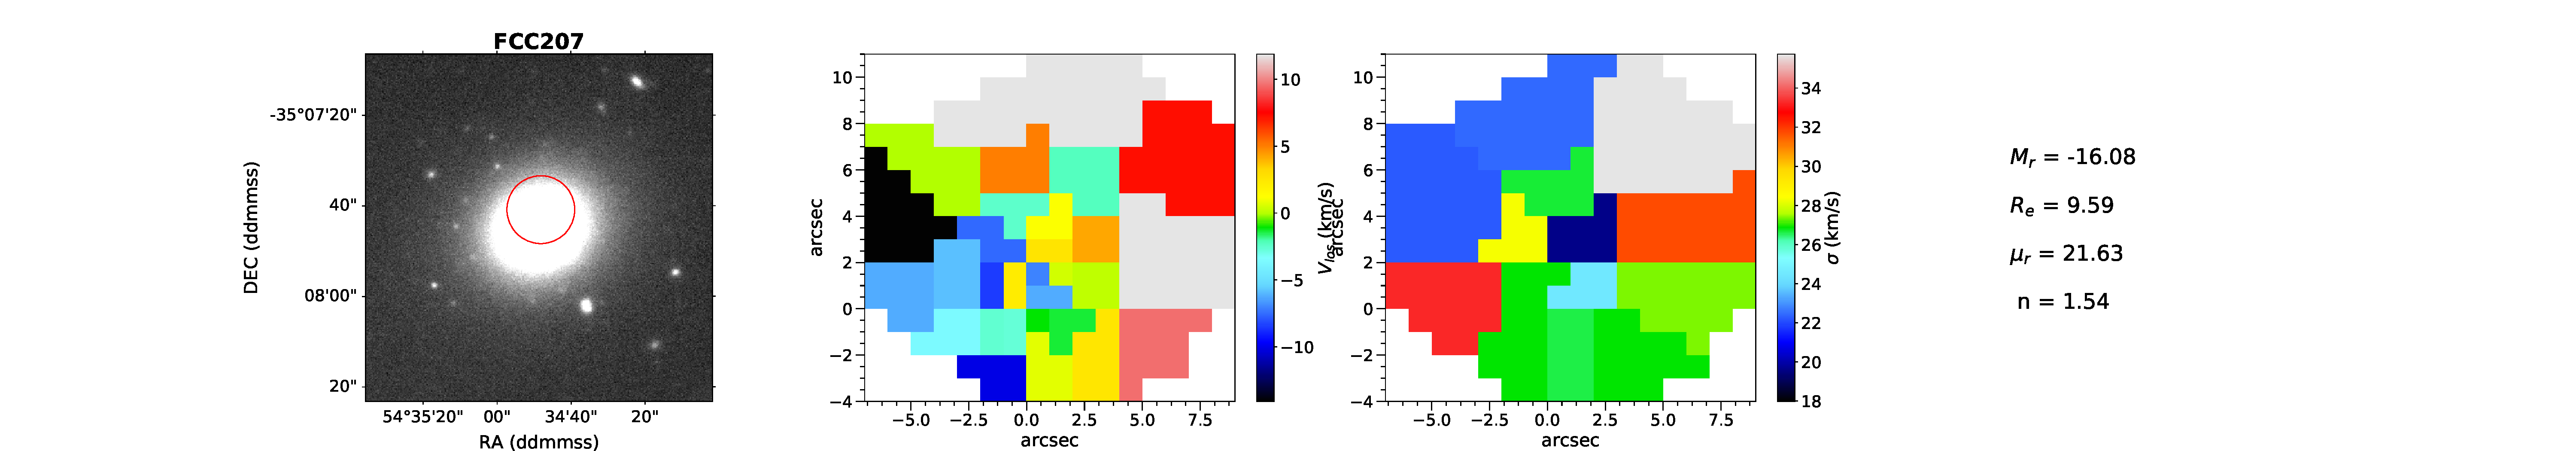
\includegraphics[width=21cm,height=6cm,keepaspectratio]{../2_pipeline/1_V&S_Maps/207Velocity_map.pdf}
         \caption{Photometric images, Velocity maps, Dispersion maps}
         \label{FigVelDis}
\end{figure*}
\clearpage
%
\begin{figure*}[!htb]
   \ContinuedFloat
   \centering
   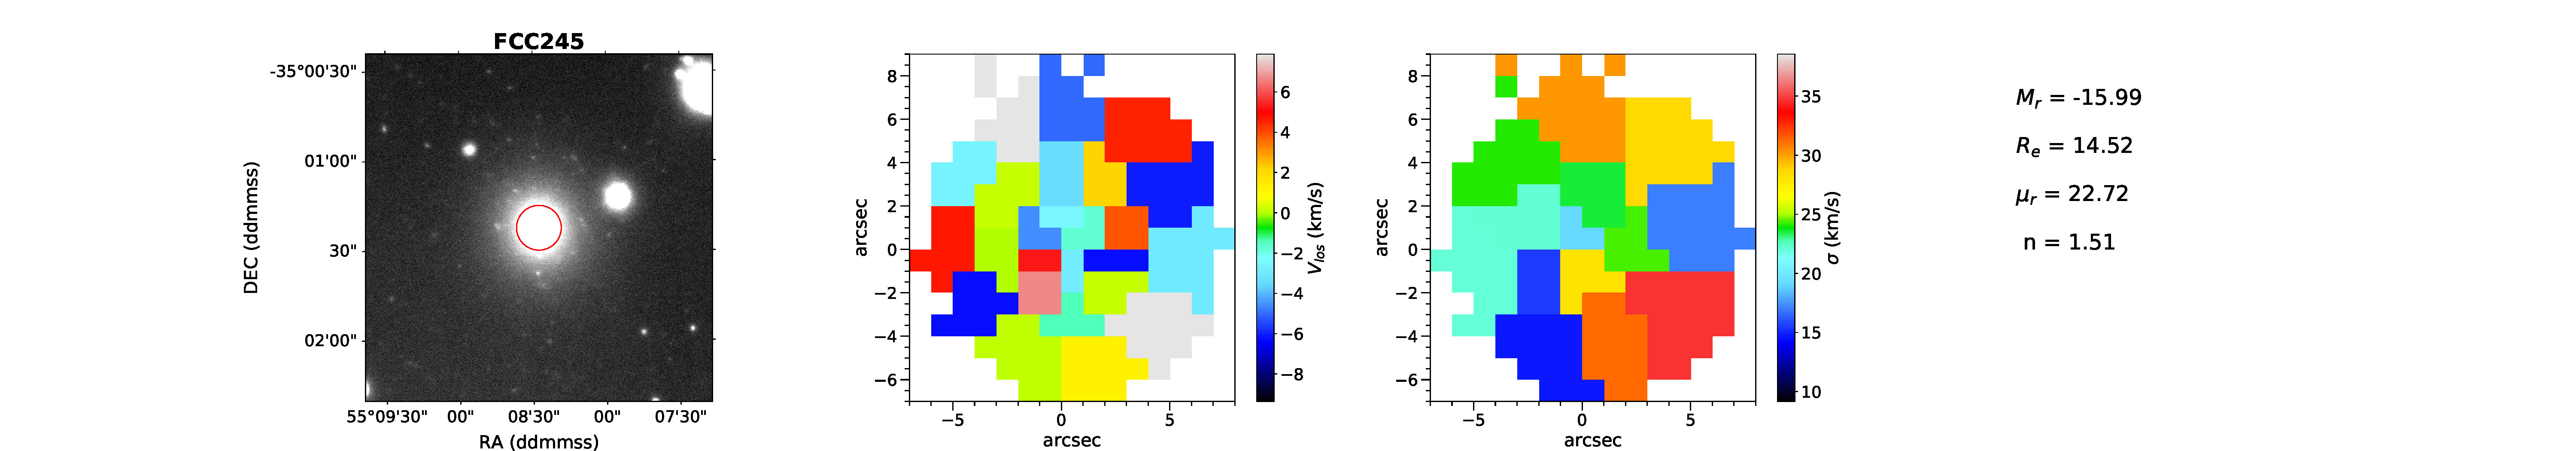
\includegraphics[width=21cm,height=6cm,keepaspectratio]{../2_pipeline/1_V&S_Maps/245Velocity_map.pdf}
   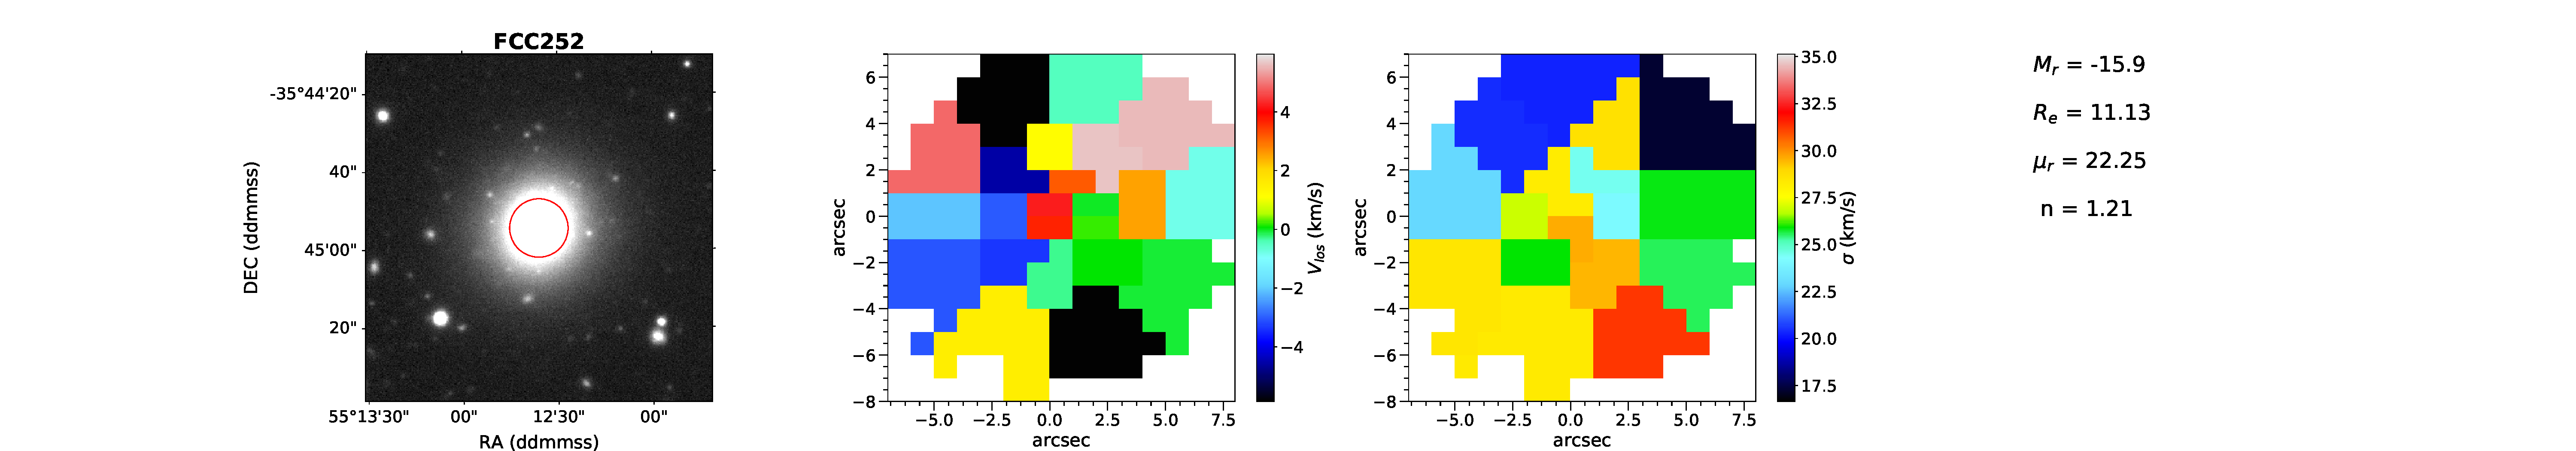
\includegraphics[width=21cm,height=6cm,keepaspectratio]{../2_pipeline/1_V&S_Maps/252Velocity_map.pdf}
   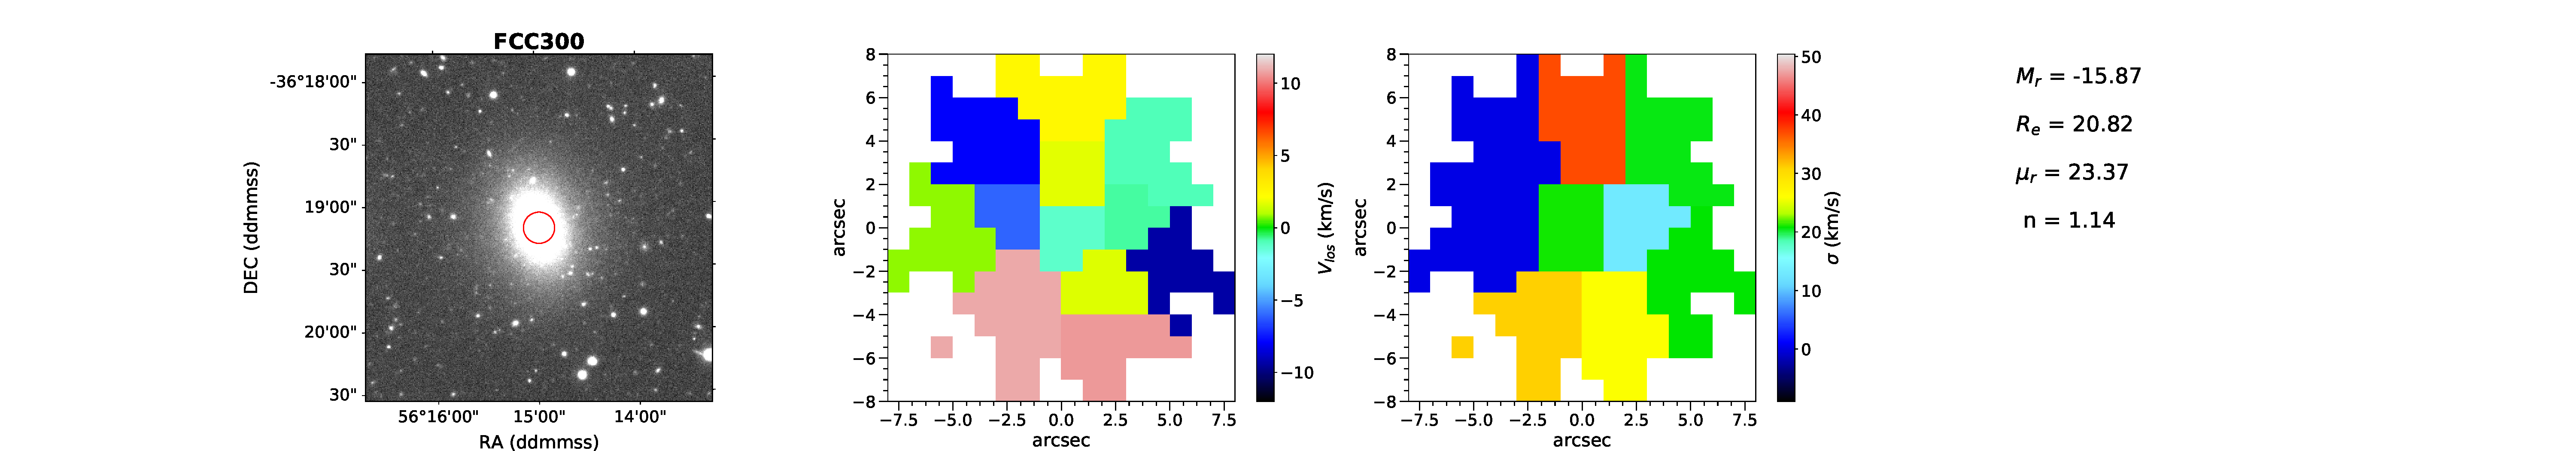
\includegraphics[width=21cm,height=6cm,keepaspectratio]{../2_pipeline/1_V&S_Maps/300Velocity_map.pdf}
   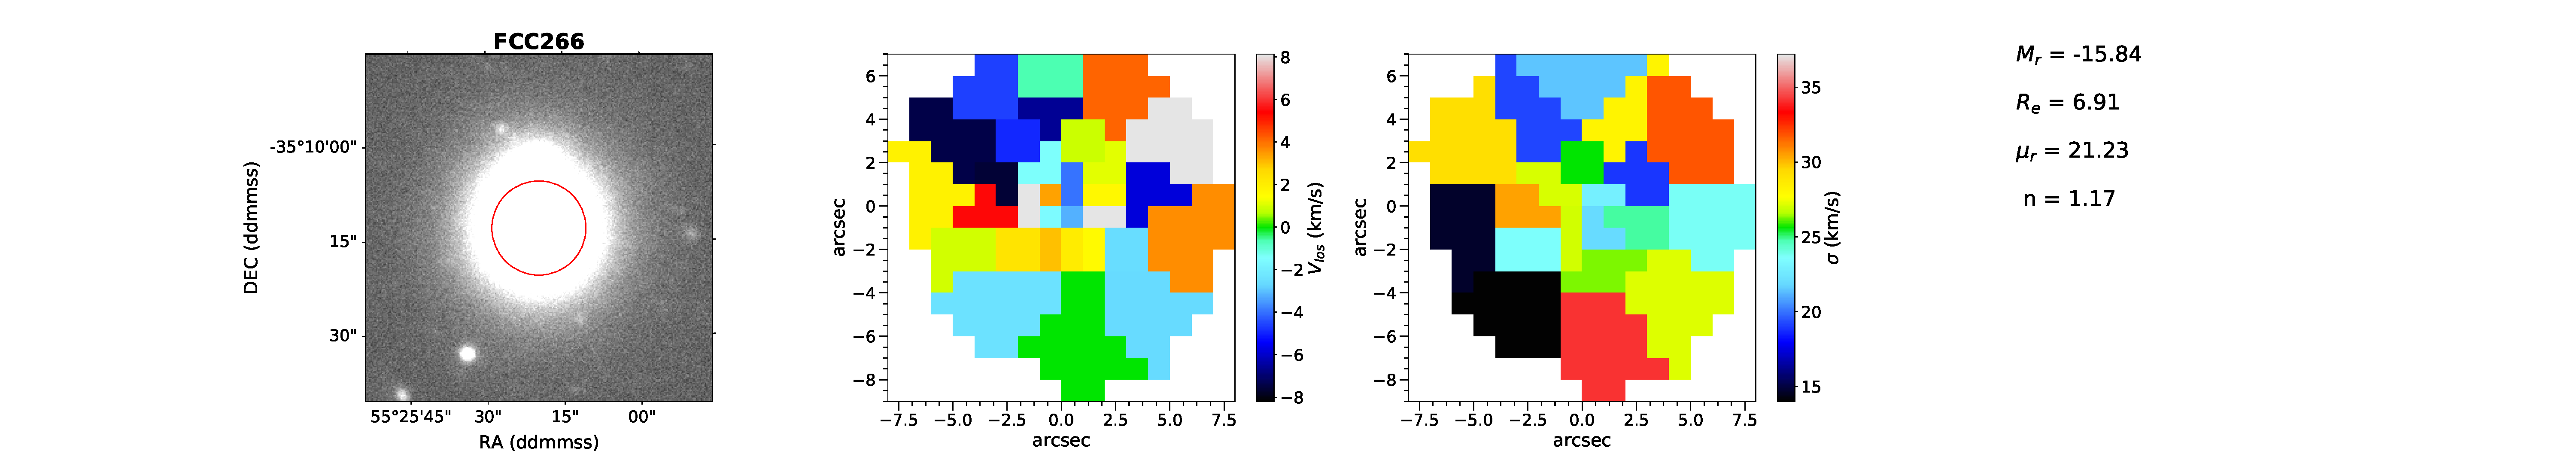
\includegraphics[width=21cm,height=6cm,keepaspectratio]{../2_pipeline/1_V&S_Maps/266Velocity_map.pdf}
   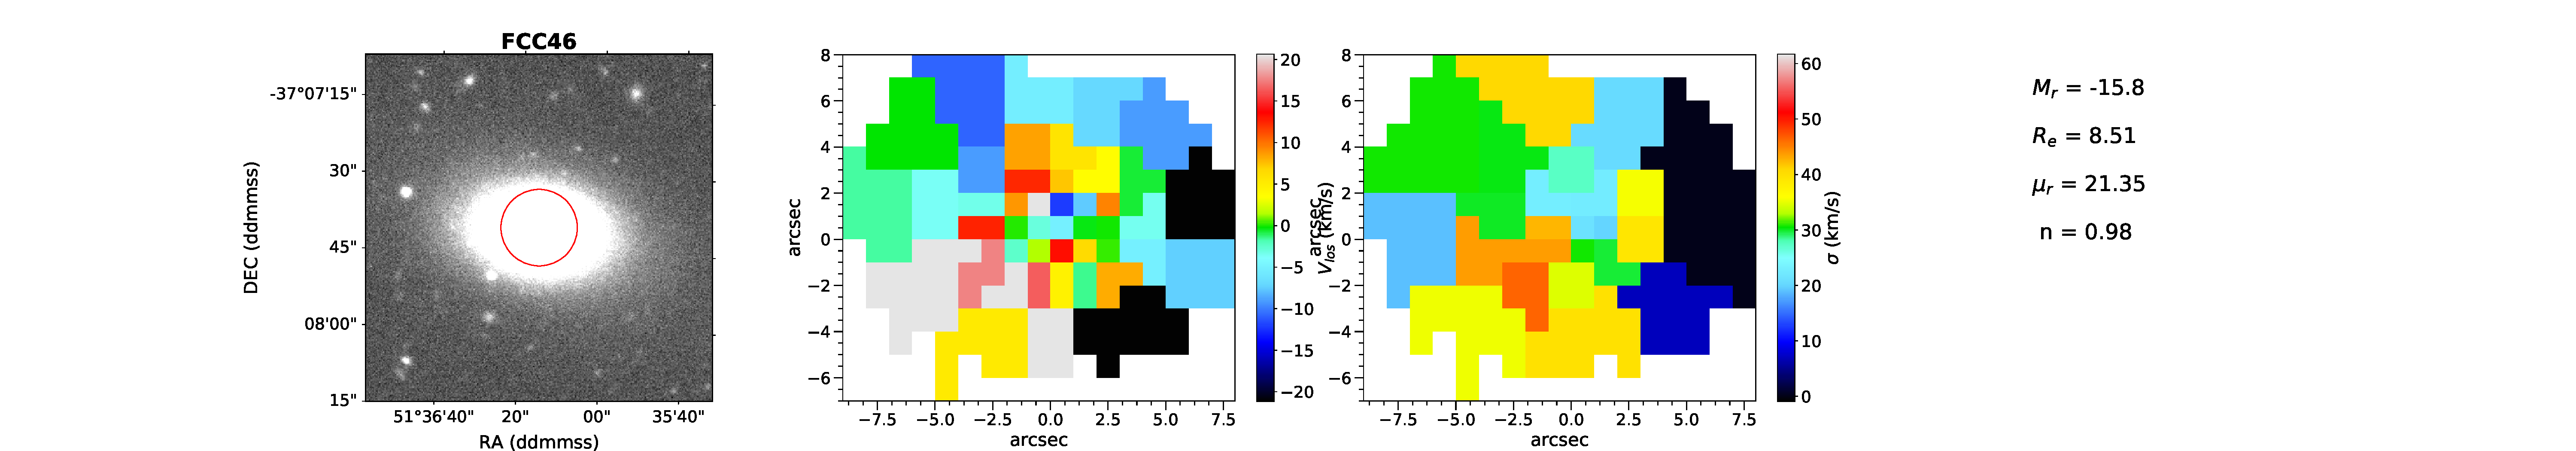
\includegraphics[width=21cm,height=6cm,keepaspectratio]{../2_pipeline/1_V&S_Maps/46Velocity_map.pdf}
   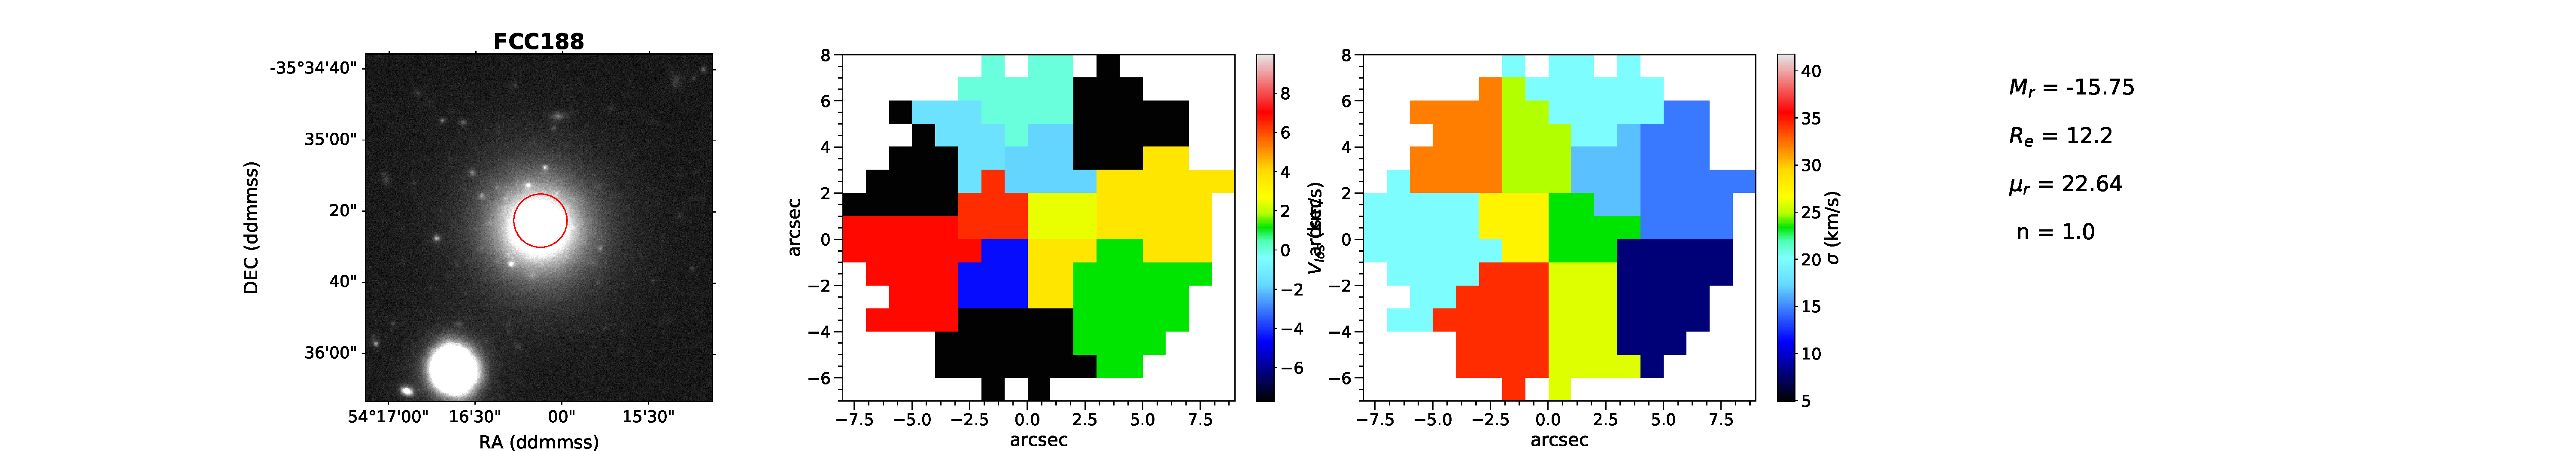
\includegraphics[width=21cm,height=6cm,keepaspectratio]{../2_pipeline/1_V&S_Maps/188Velocity_map.pdf}
         \caption{Photometric images, Velocity maps, Dispersion maps}
         \label{FigVelDis}
\end{figure*}
\clearpage
%
\begin{figure*}[!htb]
   \ContinuedFloat
   \centering
   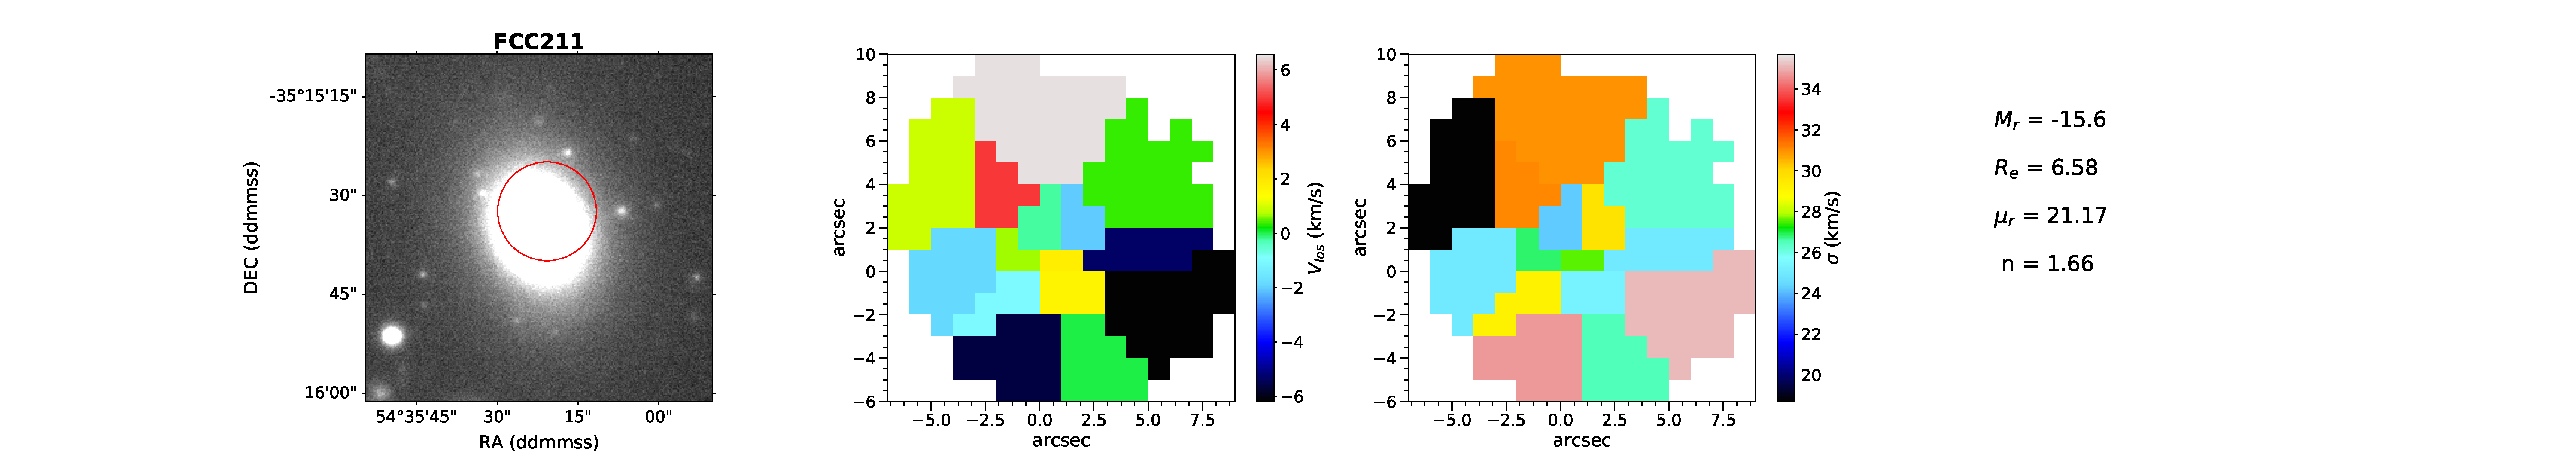
\includegraphics[width=21cm,height=6cm,keepaspectratio]{../2_pipeline/1_V&S_Maps/211Velocity_map.pdf}
   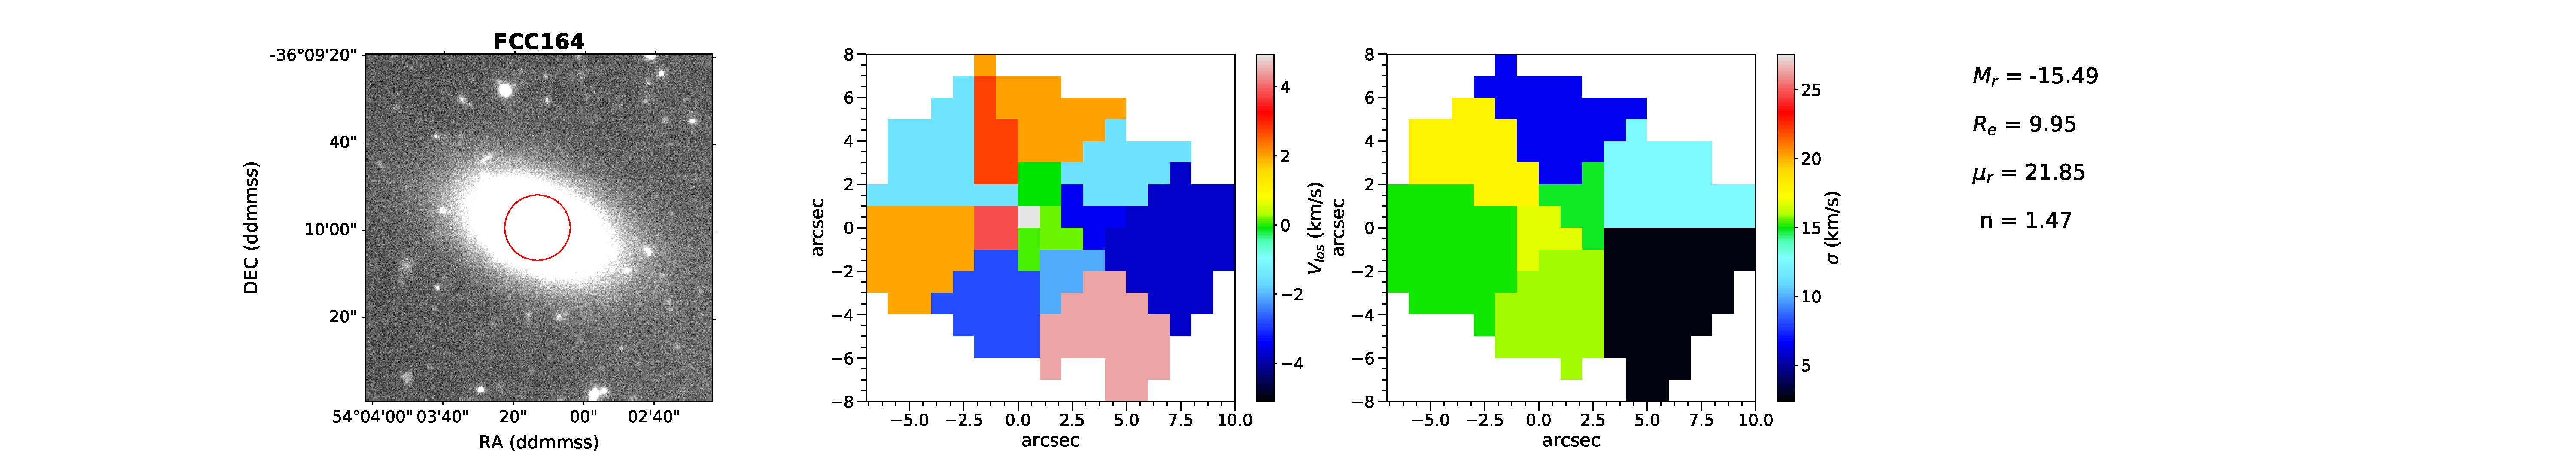
\includegraphics[width=21cm,height=6cm,keepaspectratio]{../2_pipeline/1_V&S_Maps/164Velocity_map.pdf}
   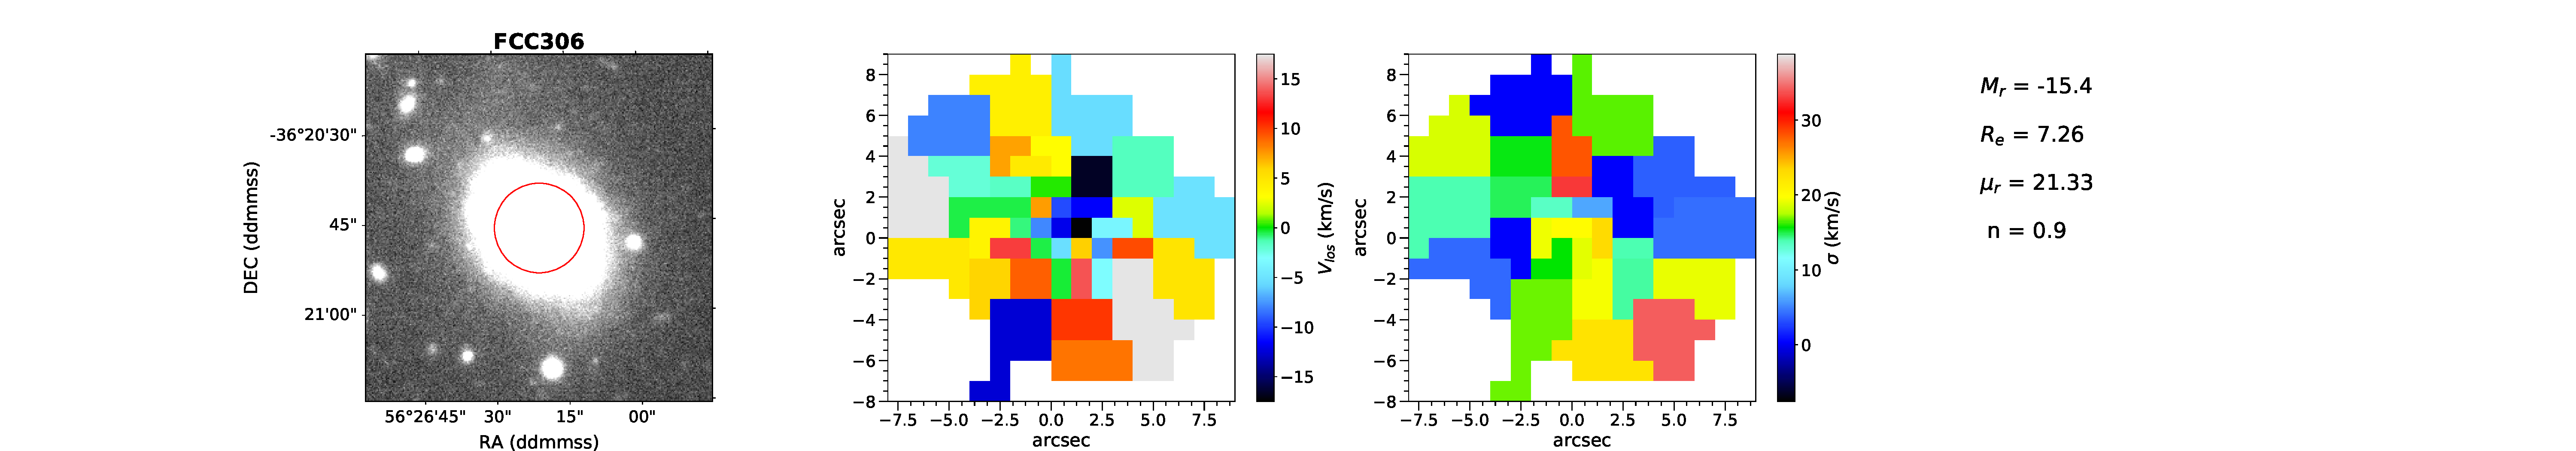
\includegraphics[width=21cm,height=6cm,keepaspectratio]{../2_pipeline/1_V&S_Maps/306Velocity_map.pdf}
   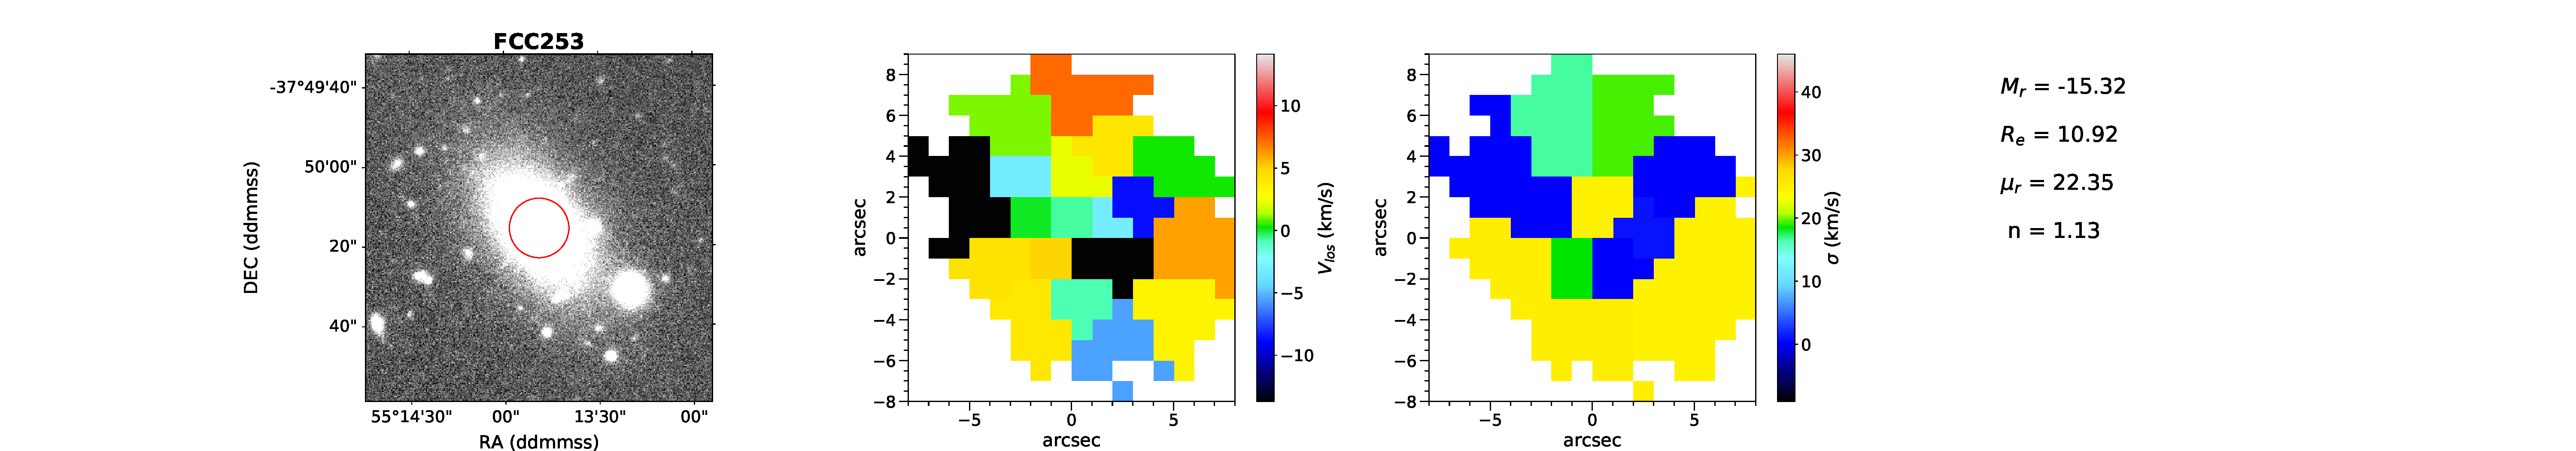
\includegraphics[width=21cm,height=6cm,keepaspectratio]{../2_pipeline/1_V&S_Maps/253Velocity_map.pdf}
   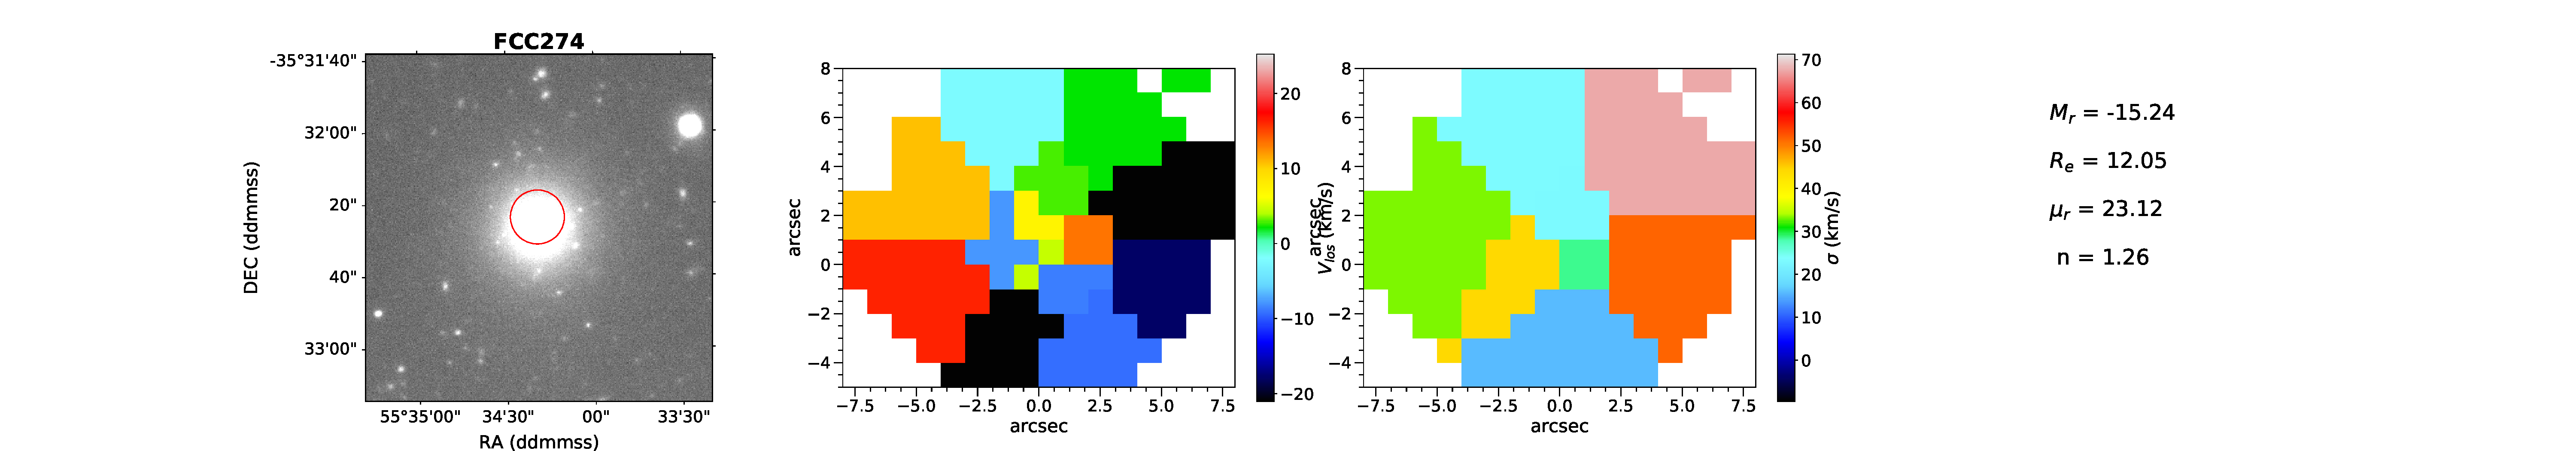
\includegraphics[width=21cm,height=6cm,keepaspectratio]{../2_pipeline/1_V&S_Maps/274Velocity_map.pdf}
   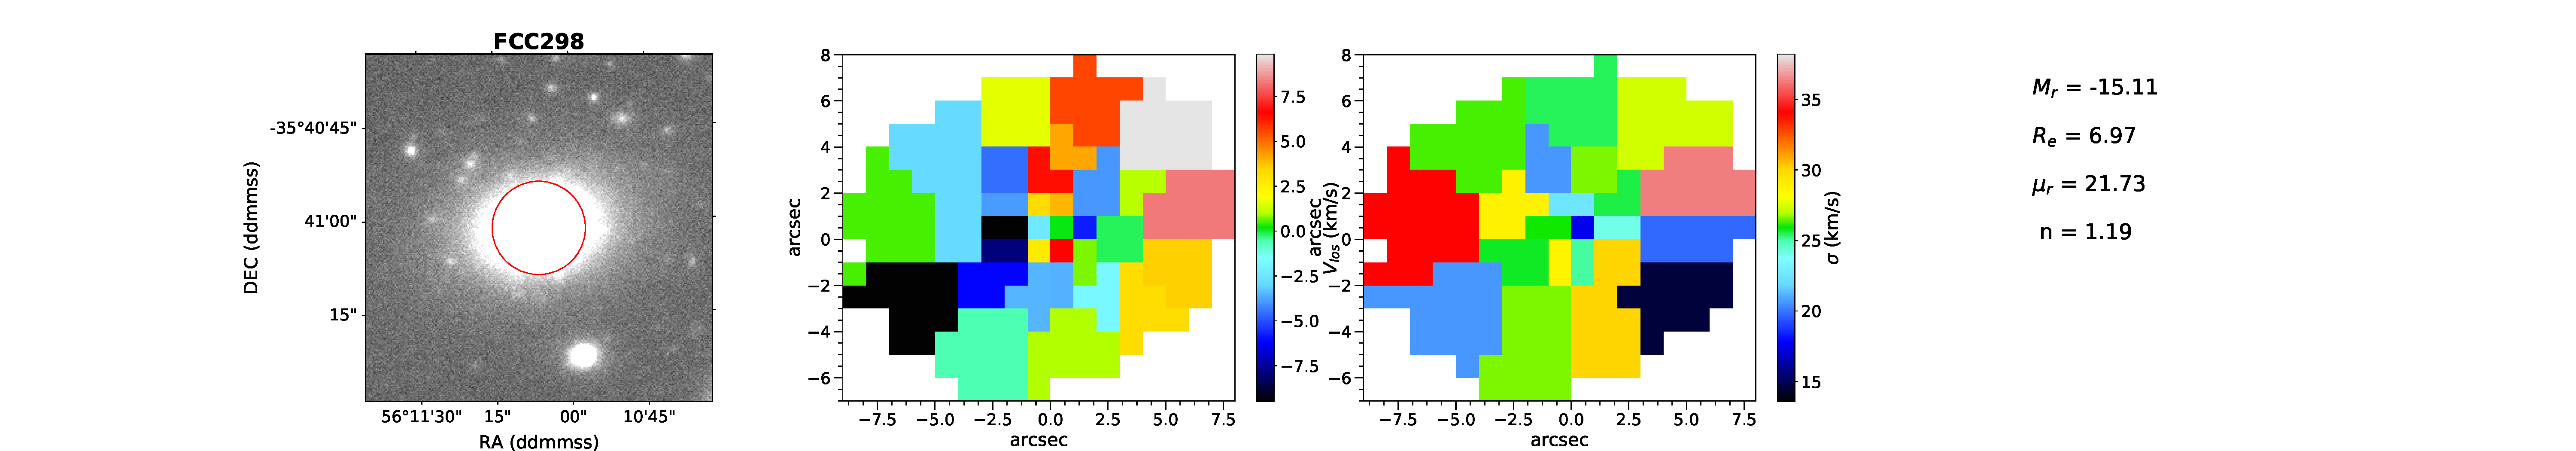
\includegraphics[width=21cm,height=6cm,keepaspectratio]{../2_pipeline/1_V&S_Maps/298Velocity_map.pdf}
         \caption{Photometric images, Velocity maps, Dispersion maps}
         \label{FigVelDis}
\end{figure*}
\clearpage
%
\begin{figure*}[!htb]
   \ContinuedFloat
   \centering
   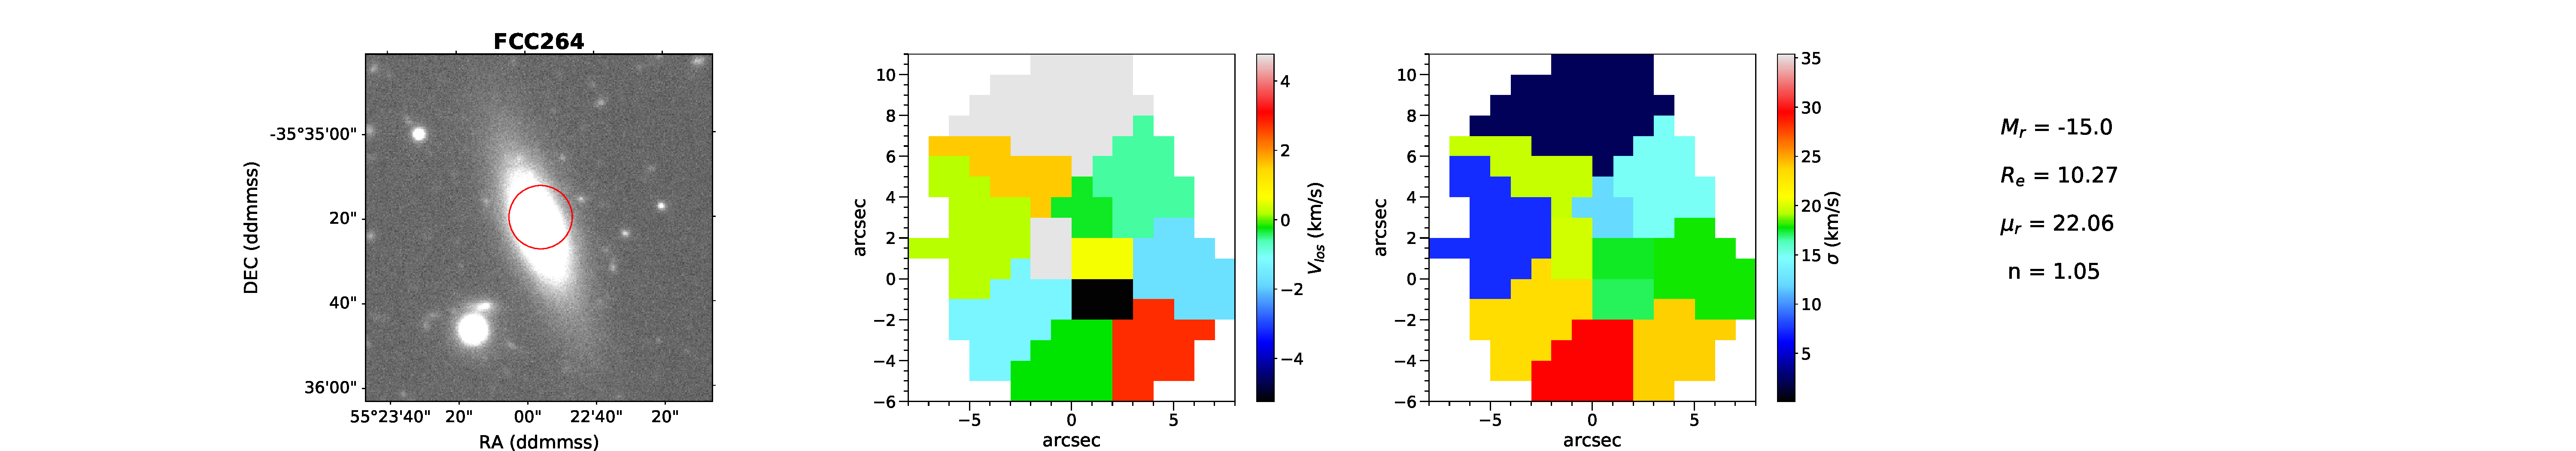
\includegraphics[width=21cm,height=6cm,keepaspectratio]{../2_pipeline/1_V&S_Maps/264Velocity_map.pdf}
   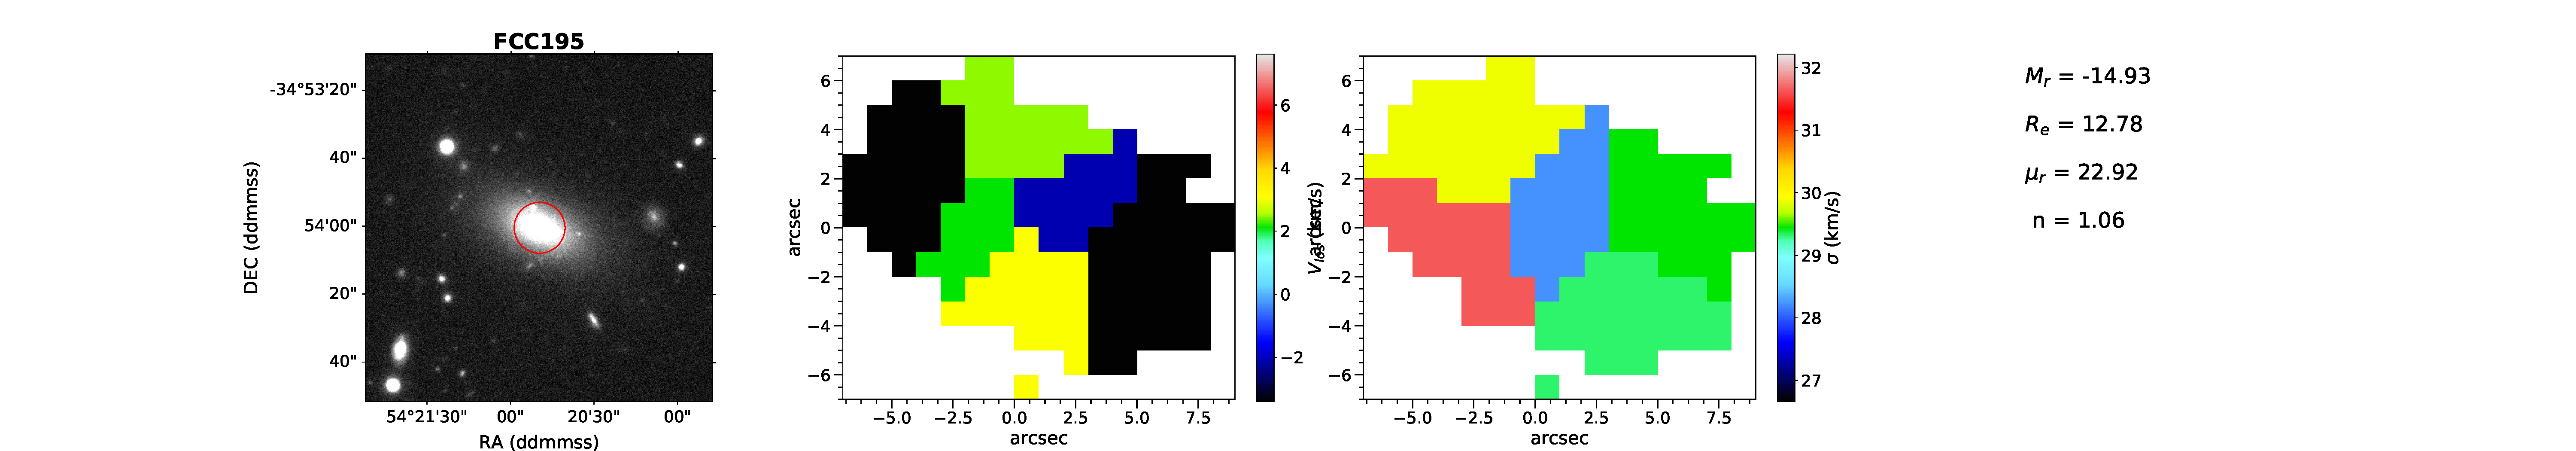
\includegraphics[width=21cm,height=6cm,keepaspectratio]{../2_pipeline/1_V&S_Maps/195Velocity_map.pdf}
   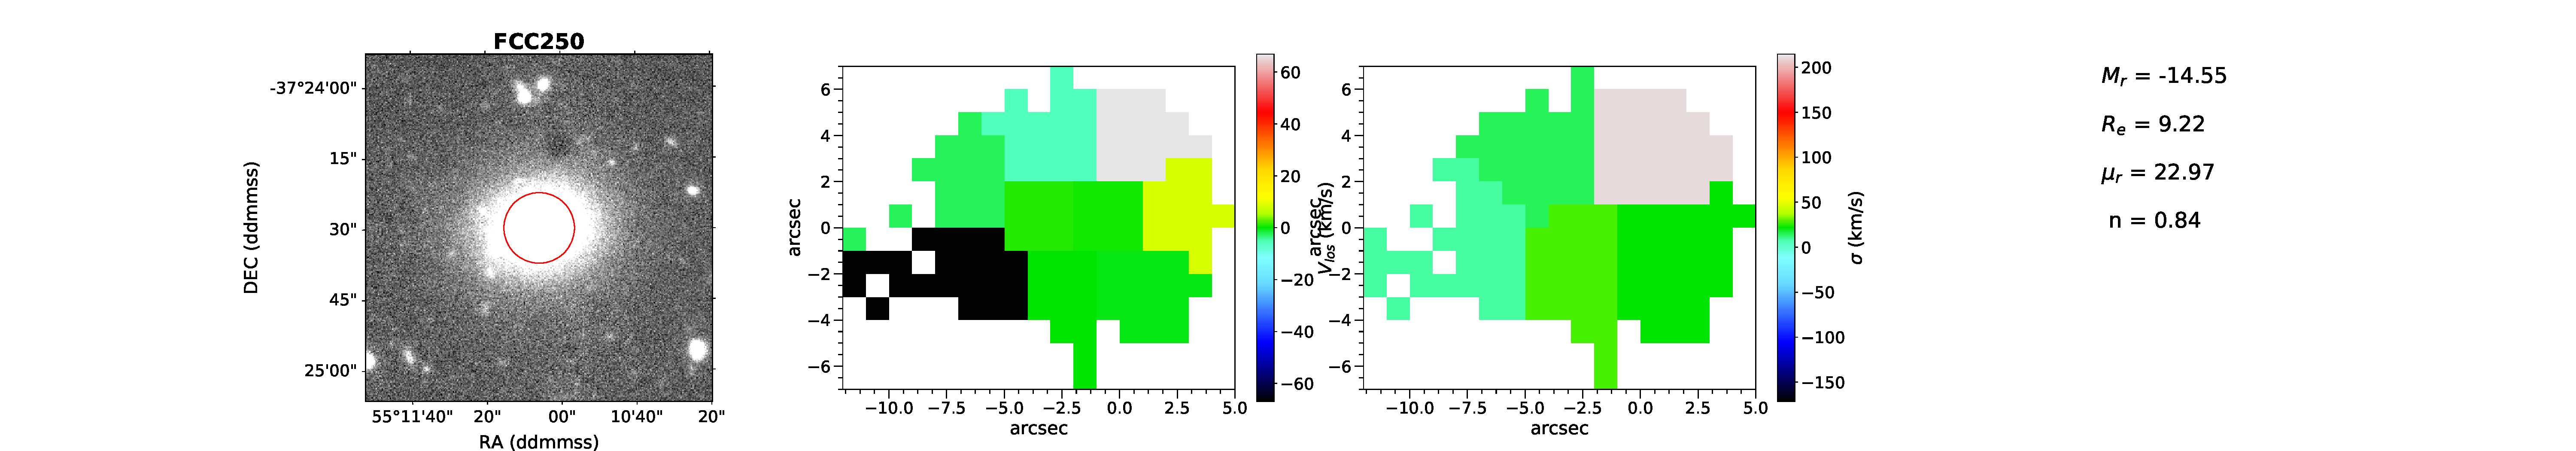
\includegraphics[width=21cm,height=6cm,keepaspectratio]{../2_pipeline/1_V&S_Maps/250Velocity_map.pdf}
   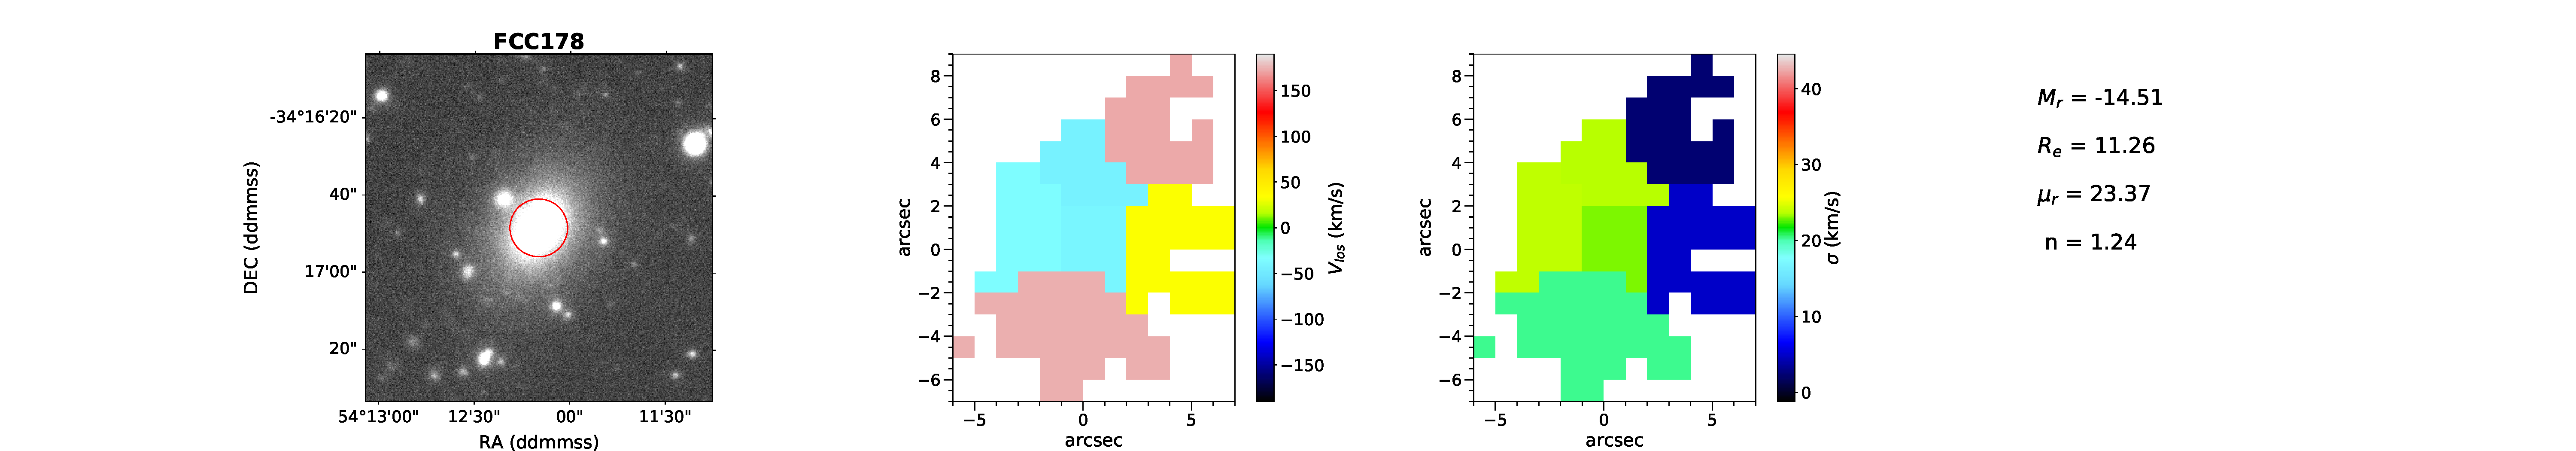
\includegraphics[width=21cm,height=6cm,keepaspectratio]{../2_pipeline/1_V&S_Maps/178Velocity_map.pdf}
   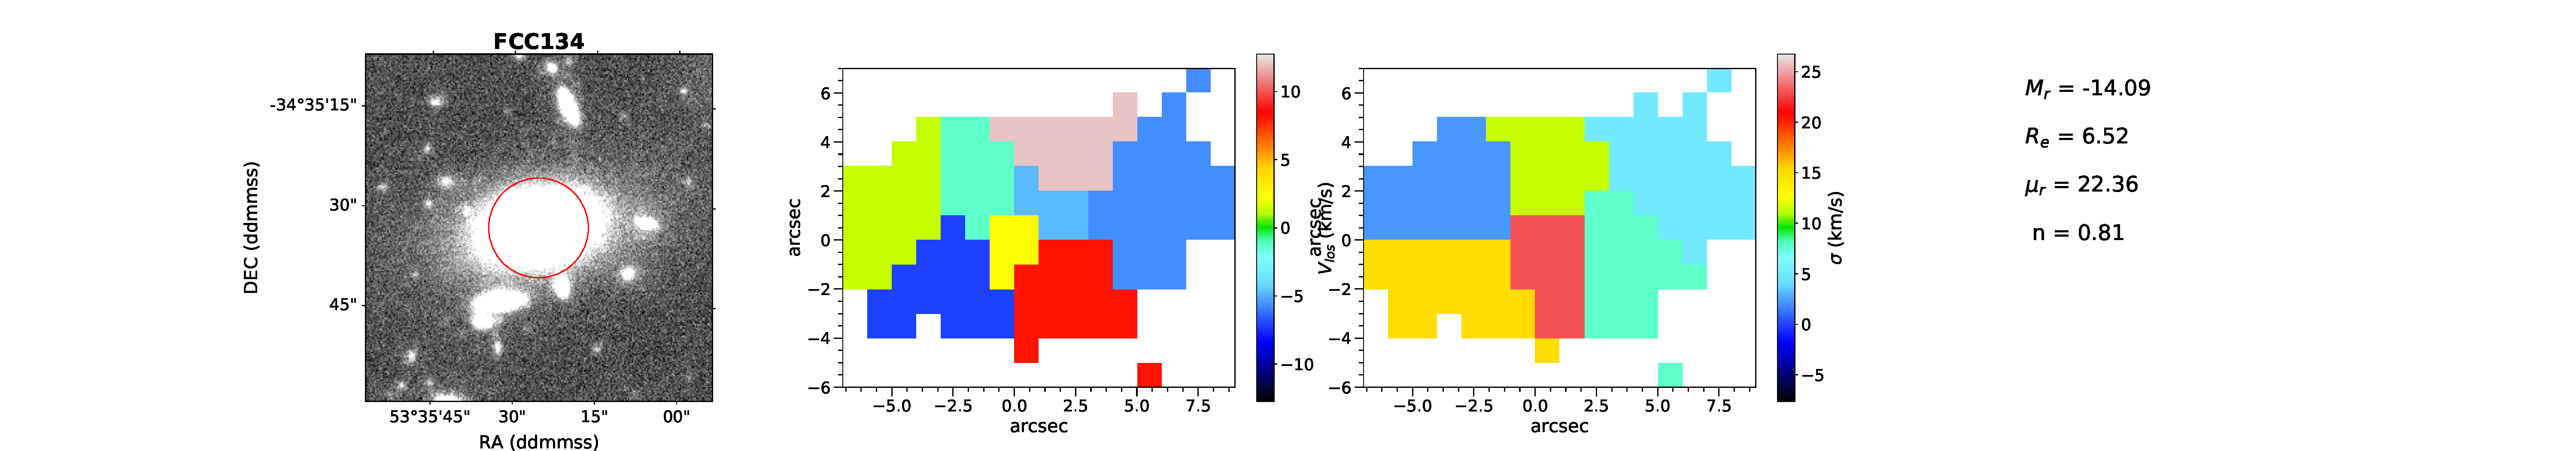
\includegraphics[width=21cm,height=6cm,keepaspectratio]{../2_pipeline/1_V&S_Maps/134Velocity_map.pdf}
	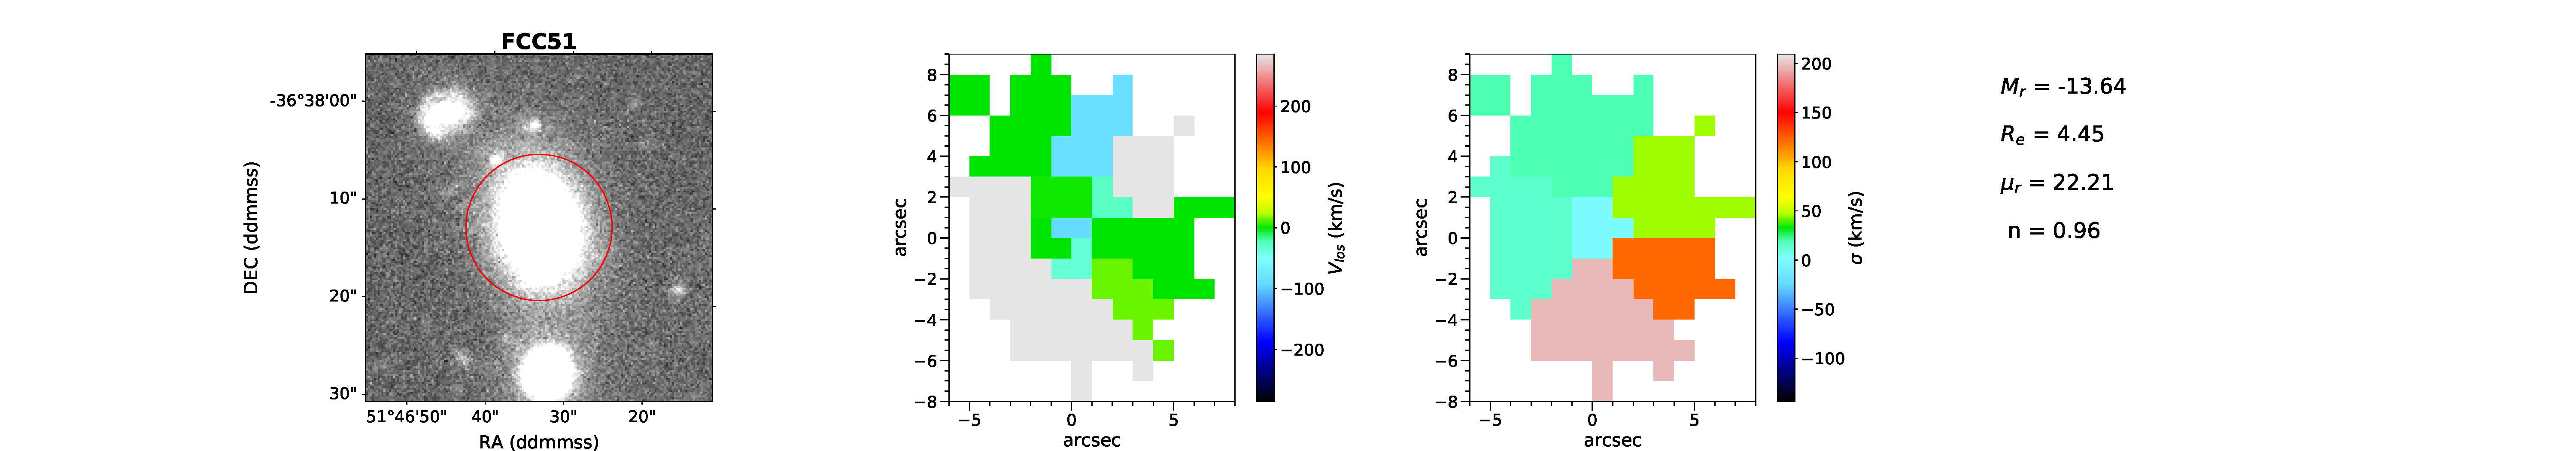
\includegraphics[width=21cm,height=6cm,keepaspectratio]{../2_pipeline/1_V&S_Maps/51Velocity_map.pdf}
         \caption{Photometric images, Velocity maps, Dispersion maps}
         \label{FigVelDis}
\end{figure*}
\clearpage
%______________________________________________________________

\section{Conclusions}

  
\begin{acknowledgements}

\end{acknowledgements}


%-------------------------------------------------------------------

\begin{thebibliography}{}

  \bibitem[1966]{baker} Baker, N. 1966,
      in Stellar Evolution,
      ed.\ R. F. Stein,\& A. G. W. Cameron
      (Plenum, New York) 333

   \bibitem[1988]{balluch} Balluch, M. 1988,
      A\&A, 200, 58

   \bibitem[1980]{cox} Cox, J. P. 1980,
      Theory of Stellar Pulsation
      (Princeton University Press, Princeton) 165

   \bibitem[1969]{cox69} Cox, A. N.,\& Stewart, J. N. 1969,
      Academia Nauk, Scientific Information 15, 1

   \bibitem[1980]{mizuno} Mizuno H. 1980,
      Prog. Theor. Phys., 64, 544
   
   \bibitem[1987]{tscharnuter} Tscharnuter W. M. 1987,
      A\&A, 188, 55
  
   \bibitem[1992]{terlevich} Terlevich, R. 1992, in ASP Conf. Ser. 31, 
      Relationships between Active Galactic Nuclei and Starburst Galaxies, 
      ed. A. V. Filippenko, 13

   \bibitem[1980a]{yorke80a} Yorke, H. W. 1980a,
      A\&A, 86, 286

   \bibitem[1997]{zheng} Zheng, W., Davidsen, A. F., Tytler, D. \& Kriss, G. A.
      1997, preprint
\end{thebibliography}

\end{document}

%%%%%%%%%%%%%%%%%%%%%%%%%%%%%%%%%%%%%%%%%%%%%%%%%%%%%%%%%%%%%%
Examples for figures using graphicx
A guide "Using Imported Graphics in LaTeX2e"  (Keith Reckdahl)
is available on a lot of LaTeX public servers or ctan mirrors.
The file is : epslatex.pdf 
%%%%%%%%%%%%%%%%%%%%%%%%%%%%%%%%%%%%%%%%%%%%%%%%%%%%%%%%%%%%%%

%_____________________________________________________________
%                 A figure as large as the width of the column
%-------------------------------------------------------------
   \begin{figure}
   \centering
   \includegraphics[width=\hsize]{empty.eps}
      \caption{Vibrational stability equation of state
               $S_{\mathrm{vib}}(\lg e, \lg \rho)$.
               $>0$ means vibrational stability.
              }
         \label{FigVibStab}
   \end{figure}
%
%_____________________________________________________________
%                                    One column rotated figure
%-------------------------------------------------------------
   \begin{figure}
   \centering
   \includegraphics[angle=-90,width=3cm]{213Velocity_map.pdf}
      \caption{Vibrational stability equation of state
               $S_{\mathrm{vib}}(\lg e, \lg \rho)$.
               $>0$ means vibrational stability.
              }
         \label{FigVibStab}
   \end{figure}
%
%_____________________________________________________________
%                        Figure with caption on the right side 
%-------------------------------------------------------------
   \begin{figure}
   \sidecaption
   \includegraphics[width=3cm]{empty.eps}
      \caption{Vibrational stability equation of state
               $S_{\mathrm{vib}}(\lg e, \lg \rho)$.
               $>0$ means vibrational stability.
              }
         \label{FigVibStab}
   \end{figure}
%
%_____________________________________________________________
%
%_____________________________________________________________
%                                Figure with a new BoundingBox 
%-------------------------------------------------------------
   \begin{figure}
   \centering
   \includegraphics[bb=10 20 100 300,width=3cm,clip]{empty.eps}
      \caption{Vibrational stability equation of state
               $S_{\mathrm{vib}}(\lg e, \lg \rho)$.
               $>0$ means vibrational stability.
              }
         \label{FigVibStab}
   \end{figure}
%
%_____________________________________________________________
%
%_____________________________________________________________
%                                      The "resizebox" command 
%-------------------------------------------------------------
   \begin{figure}
   \resizebox{\hsize}{!}
            {\includegraphics[bb=10 20 100 300,clip]{empty.eps}
      \caption{Vibrational stability equation of state
               $S_{\mathrm{vib}}(\lg e, \lg \rho)$.
               $>0$ means vibrational stability.
              }}
         \label{FigVibStab}
   \end{figure}
%
%______________________________________________________________
%
%_____________________________________________________________
%                                             Two column Figure 
%-------------------------------------------------------------
   \begin{figure*}
   \resizebox{\hsize}{!}
           {\includegraphics[bb=10 20 100 300,clip]{213Velocity_map.pdf}
      \caption{Vibrational stability equation of state
               $S_{\mathrm{vib}}(\lg e, \lg \rho)$.
               $>0$ means vibrational stability.
              }}
         \label{FigVibStab}
   \end{figure*}
%
%______________________________________________________________
%
%_____________________________________________________________
%                                             Simple A&A Table
%_____________________________________________________________
%
\begin{table}
\caption{Nonlinear Model Results}             % title of Table
\label{table:1}      % is used to refer this table in the text
\centering                          % used for centering table
\begin{tabular}{c c c c}        % centered columns (4 columns)
\hline\hline                 % inserts double horizontal lines
HJD & $E$ & Method\#2 & Method\#3 \\    % table heading 
\hline                        % inserts single horizontal line
   1 & 50 & $-837$ & 970 \\      % inserting body of the table
   2 & 47 & 877    & 230 \\
   3 & 31 & 25     & 415 \\
   4 & 35 & 144    & 2356 \\
   5 & 45 & 300    & 556 \\ 
\hline                                   %inserts single line
\end{tabular}
\end{table}
%
%_____________________________________________________________
%                                             Two column Table 
%_____________________________________________________________
%
\begin{table*}
\caption{Nonlinear Model Results}             
\label{table:1}      
\centering          
\begin{tabular}{c c c c l l l }     % 7 columns 
\hline\hline       
                      % To combine 4 columns into a single one 
HJD & $E$ & Method\#2 & \multicolumn{4}{c}{Method\#3}\\ 
\hline                    
   1 & 50 & $-837$ & 970 & 65 & 67 & 78\\  
   2 & 47 & 877    & 230 & 567& 55 & 78\\
   3 & 31 & 25     & 415 & 567& 55 & 78\\
   4 & 35 & 144    & 2356& 567& 55 & 78 \\
   5 & 45 & 300    & 556 & 567& 55 & 78\\
\hline                  
\end{tabular}
\end{table*}
%
%-------------------------------------------------------------
%                                          Table with notes 
%-------------------------------------------------------------
%
% A single note
\begin{table}
\caption{\label{t7}Spectral types and photometry for stars in the
  region.}
\centering
\begin{tabular}{lccc}
\hline\hline
Star&Spectral type&RA(J2000)&Dec(J2000)\\
\hline
69           &B1\,V     &09 15 54.046 & $-$50 00 26.67\\
49           &B0.7\,V   &*09 15 54.570& $-$50 00 03.90\\
LS~1267~(86) &O8\,V     &09 15 52.787&11.07\\
24.6         &7.58      &1.37 &0.20\\
\hline
LS~1262      &B0\,V     &09 15 05.17&11.17\\
MO 2-119     &B0.5\,V   &09 15 33.7 &11.74\\
LS~1269      &O8.5\,V   &09 15 56.60&10.85\\
\hline
\end{tabular}
\tablefoot{The top panel shows likely members of Pismis~11. The second
panel contains likely members of Alicante~5. The bottom panel
displays stars outside the clusters.}
\end{table}
%
% More notes
%
\begin{table}
\caption{\label{t7}Spectral types and photometry for stars in the
  region.}
\centering
\begin{tabular}{lccc}
\hline\hline
Star&Spectral type&RA(J2000)&Dec(J2000)\\
\hline
69           &B1\,V     &09 15 54.046 & $-$50 00 26.67\\
49           &B0.7\,V   &*09 15 54.570& $-$50 00 03.90\\
LS~1267~(86) &O8\,V     &09 15 52.787&11.07\tablefootmark{a}\\
24.6         &7.58\tablefootmark{1}&1.37\tablefootmark{a}   &0.20\tablefootmark{a}\\
\hline
LS~1262      &B0\,V     &09 15 05.17&11.17\tablefootmark{b}\\
MO 2-119     &B0.5\,V   &09 15 33.7 &11.74\tablefootmark{c}\\
LS~1269      &O8.5\,V   &09 15 56.60&10.85\tablefootmark{d}\\
\hline
\end{tabular}
\tablefoot{The top panel shows likely members of Pismis~11. The second
panel contains likely members of Alicante~5. The bottom panel
displays stars outside the clusters.\\
\tablefoottext{a}{Photometry for MF13, LS~1267 and HD~80077 from
Dupont et al.}
\tablefoottext{b}{Photometry for LS~1262, LS~1269 from
Durand et al.}
\tablefoottext{c}{Photometry for MO2-119 from
Mathieu et al.}
}
\end{table}
%
%-------------------------------------------------------------
%                                       Table with references 
%-------------------------------------------------------------
%
\begin{table*}[h]
 \caption[]{\label{nearbylistaa2}List of nearby SNe used in this work.}
\begin{tabular}{lccc}
 \hline \hline
  SN name &
  Epoch &
 Bands &
  References \\
 &
  (with respect to $B$ maximum) &
 &
 \\ \hline
1981B   & 0 & {\it UBV} & 1\\
1986G   &  $-$3, $-$1, 0, 1, 2 & {\it BV}  & 2\\
1989B   & $-$5, $-$1, 0, 3, 5 & {\it UBVRI}  & 3, 4\\
1990N   & 2, 7 & {\it UBVRI}  & 5\\
1991M   & 3 & {\it VRI}  & 6\\
\hline
\noalign{\smallskip}
\multicolumn{4}{c}{ SNe 91bg-like} \\
\noalign{\smallskip}
\hline
1991bg   & 1, 2 & {\it BVRI}  & 7\\
1999by   & $-$5, $-$4, $-$3, 3, 4, 5 & {\it UBVRI}  & 8\\
\hline
\noalign{\smallskip}
\multicolumn{4}{c}{ SNe 91T-like} \\
\noalign{\smallskip}
\hline
1991T   & $-$3, 0 & {\it UBVRI}  &  9, 10\\
2000cx  & $-$3, $-$2, 0, 1, 5 & {\it UBVRI}  & 11\\ %
\hline
\end{tabular}
\tablebib{(1)~\citet{branch83};
(2) \citet{phillips87}; (3) \citet{barbon90}; (4) \citet{wells94};
(5) \citet{mazzali93}; (6) \citet{gomez98}; (7) \citet{kirshner93};
(8) \citet{patat96}; (9) \citet{salvo01}; (10) \citet{branch03};
(11) \citet{jha99}.
}
\end{table*}
%_____________________________________________________________
%                      A rotated Two column Table in landscape  
%-------------------------------------------------------------
\begin{sidewaystable*}
\caption{Summary for ISOCAM sources with mid-IR excess 
(YSO candidates).}\label{YSOtable}
\centering
\begin{tabular}{crrlcl} 
\hline\hline             
ISO-L1551 & $F_{6.7}$~[mJy] & $\alpha_{6.7-14.3}$ 
& YSO type$^{d}$ & Status & Comments\\
\hline
  \multicolumn{6}{c}{\it New YSO candidates}\\ % To combine 6 columns into a single one
\hline
  1 & 1.56 $\pm$ 0.47 & --    & Class II$^{c}$ & New & Mid\\
  2 & 0.79:           & 0.97: & Class II ?     & New & \\
  3 & 4.95 $\pm$ 0.68 & 3.18  & Class II / III & New & \\
  5 & 1.44 $\pm$ 0.33 & 1.88  & Class II       & New & \\
\hline
  \multicolumn{6}{c}{\it Previously known YSOs} \\
\hline
  61 & 0.89 $\pm$ 0.58 & 1.77 & Class I & \object{HH 30} & Circumstellar disk\\
  96 & 38.34 $\pm$ 0.71 & 37.5& Class II& MHO 5          & Spectral type\\
\hline
\end{tabular}
\end{sidewaystable*}
%_____________________________________________________________
%                      A rotated One column Table in landscape  
%-------------------------------------------------------------
\begin{sidewaystable}
\caption{Summary for ISOCAM sources with mid-IR excess 
(YSO candidates).}\label{YSOtable}
\centering
\begin{tabular}{crrlcl} 
\hline\hline             
ISO-L1551 & $F_{6.7}$~[mJy] & $\alpha_{6.7-14.3}$ 
& YSO type$^{d}$ & Status & Comments\\
\hline
  \multicolumn{6}{c}{\it New YSO candidates}\\ % To combine 6 columns into a single one
\hline
  1 & 1.56 $\pm$ 0.47 & --    & Class II$^{c}$ & New & Mid\\
  2 & 0.79:           & 0.97: & Class II ?     & New & \\
  3 & 4.95 $\pm$ 0.68 & 3.18  & Class II / III & New & \\
  5 & 1.44 $\pm$ 0.33 & 1.88  & Class II       & New & \\
\hline
  \multicolumn{6}{c}{\it Previously known YSOs} \\
\hline
  61 & 0.89 $\pm$ 0.58 & 1.77 & Class I & \object{HH 30} & Circumstellar disk\\
  96 & 38.34 $\pm$ 0.71 & 37.5& Class II& MHO 5          & Spectral type\\
\hline
\end{tabular}
\end{sidewaystable}
%
%_____________________________________________________________
%                              Table longer than a single page  
%-------------------------------------------------------------
% All long tables will be placed automatically at the end, after 
%                                        \end{thebibliography}
%
\begin{longtab}
\begin{longtable}{lllrrr}
\caption{\label{kstars} Sample stars with absolute magnitude}\\
\hline\hline
Catalogue& $M_{V}$ & Spectral & Distance & Mode & Count Rate \\
\hline
\endfirsthead
\caption{continued.}\\
\hline\hline
Catalogue& $M_{V}$ & Spectral & Distance & Mode & Count Rate \\
\hline
\endhead
\hline
\endfoot
%%
Gl 33    & 6.37 & K2 V & 7.46 & S & 0.043170\\
Gl 66AB  & 6.26 & K2 V & 8.15 & S & 0.260478\\
Gl 68    & 5.87 & K1 V & 7.47 & P & 0.026610\\
         &      &      &      & H & 0.008686\\
Gl 86 
\footnote{Source not included in the HRI catalog. See Sect.~5.4.2 for details.}
         & 5.92 & K0 V & 10.91& S & 0.058230\\
\end{longtable}
\end{longtab}
%
%_____________________________________________________________
%                              Table longer than a single page
%                                             and in landscape 
%  In the preamble, use:       \usepackage{lscape}
%-------------------------------------------------------------
% All long tables will be placed automatically at the end, after
%                                        \end{thebibliography}
%
\begin{longtab}
\begin{landscape}
\begin{longtable}{lllrrr}
\caption{\label{kstars} Sample stars with absolute magnitude}\\
\hline\hline
Catalogue& $M_{V}$ & Spectral & Distance & Mode & Count Rate \\
\hline
\endfirsthead
\caption{continued.}\\
\hline\hline
Catalogue& $M_{V}$ & Spectral & Distance & Mode & Count Rate \\
\hline
\endhead
\hline
\endfoot
%%
Gl 33    & 6.37 & K2 V & 7.46 & S & 0.043170\\
Gl 66AB  & 6.26 & K2 V & 8.15 & S & 0.260478\\
Gl 68    & 5.87 & K1 V & 7.47 & P & 0.026610\\
         &      &      &      & H & 0.008686\\
Gl 86
\footnote{Source not included in the HRI catalog. See Sect.~5.4.2 for details.}
         & 5.92 & K0 V & 10.91& S & 0.058230\\
\end{longtable}
\end{landscape}
\end{longtab}
%
% Online Material
%_____________________________________________________________
%        Online appendices have to be placed at the end, after
%                                        \end{thebibliography}
%-------------------------------------------------------------
%\end{thebibliography}

\Online

\begin{appendix} %First online appendix
\section{Background galaxy number counts and shear noise-levels}
Because the optical images used in this analysis...

\begin{figure*}
\centering
\includegraphics[width=16.4cm,clip]{1787f24.ps}
\caption{Plotted above...}
\label{appfig}
\end{figure*}

Because the optical images...
\end{appendix}

\begin{appendix} %Second online appendix
These studies, however, have faced...
\end{appendix}

%\end{document}
%
%_____________________________________________________________
%        Some tables or figures are in the printed version and
%                      some are only in the electronic version
%-------------------------------------------------------------
%
% Leave all the tables or figures in the text, at their right place 
% and use the commands \onlfig{} and \onltab{}. These elements
% will be automatically placed at the end, in the section
% Online material.

\documentclass{aa}
...
\begin{document}
text of the paper...
\begin{figure*}%f1
\includegraphics[width=10.9cm]{1787f01.eps}
\caption{Shown in greyscale is a...}
\label{cl12301}
\end{figure*}
...
from the intrinsic ellipticity distribution.
% Figure 2 available electronically only
\onlfig{
\begin{figure*}%f2
\includegraphics[width=11.6cm]{1787f02.eps}
\caption {Shown in greyscale...}
\label{cl1018}
\end{figure*}
}

% Figure 3 available electronically only
\onlfig{
\begin{figure*}%f3
\includegraphics[width=11.2cm]{1787f03.eps}
\caption{Shown in panels...}
\label{cl1059}
\end{figure*}
}

\begin{figure*}%f4
\includegraphics[width=10.9cm]{1787f04.eps}
\caption{Shown in greyscale is...}
\label{cl1232}
\end{figure*}

\begin{table}%t1
\caption{Complexes characterisation.}\label{starbursts}
\centering
\begin{tabular}{lccc}
\hline \hline
Complex & $F_{60}$ & 8.6 &  No. of  \\
...
\hline
\end{tabular}
\end{table}
The second method produces...

% Figure 5 available electronically only
\onlfig{
\begin{figure*}%f5
\includegraphics[width=11.2cm]{1787f05.eps}
\caption{Shown in panels...}
\label{cl1238}
\end{figure*}
}

As can be seen, in general the deeper...
% Table 2 available electronically only
\onltab{
\begin{table*}%t2
\caption{List of the LMC stellar complexes...}\label{Properties}
\centering
\begin{tabular}{lccccccccc}
\hline  \hline
Stellar & RA & Dec & ...
...
\hline
\end{tabular}
\end{table*}
}

% Table 3 available electronically only
\onltab{
\begin{table*}%t3
\caption{List of the derived...}\label{IrasFluxes}
\centering
\begin{tabular}{lcccccccccc}
\hline \hline
Stellar & $f12$ & $L12$ &...
...
\hline
\end{tabular}
\end{table*}
}
\end{document}
%
%-------------------------------------------------------------
%     For the online material, table longer than a single page
%                 In the preamble for landscape case, use : 
%                                          \usepackage{lscape}
%-------------------------------------------------------------
\documentclass{aa}
\usepackage[varg]{txfonts}
\usepackage{graphicx}
\usepackage{lscape}

\begin{document}
text of the paper
% Table will be print automatically at the end, in the section Online material.
\onllongtab{
\begin{longtable}{lrcrrrrrrrrl}
\caption{Line data and abundances ...}\\
\hline
\hline
Def & mol & Ion & $\lambda$ & $\chi$ & $\log gf$ & N & e &  rad & $\delta$ & $\delta$ 
red & References \\
\hline
\endfirsthead
\caption{Continued.} \\
\hline
Def & mol & Ion & $\lambda$ & $\chi$ & $\log gf$ & B & C &  rad & $\delta$ & $\delta$ 
red & References \\
\hline
\endhead
\hline
\endfoot
\hline
\endlastfoot
A & CH & 1 &3638 & 0.002 & $-$2.551 &  &  &  & $-$150 & 150 &  Jorgensen et al. (1996) \\                    
\end{longtable}
}% End onllongtab

% Or for landscape, large table:

\onllongtab{
\begin{landscape}
\begin{longtable}{lrcrrrrrrrrl}
...
\end{longtable}
\end{landscape}
}% End onllongtab
\end{document}